\documentclass[specialist, subf, href, colorlinks=true, 14pt, times, mtpro, final]{disser}

\usepackage[utf8x]{inputenc}
\usepackage[english, russian]{babel}
\usepackage[T2A]{fontenc}
\usepackage{amsmath,amsthm,amssymb}
\usepackage {wrapfig}
\usepackage {enumitem}  
\usepackage{graphicx}
\usepackage{multicol}
\usepackage{mathrsfs}
\usepackage{xcolor}
\usepackage{hyperref}
\usepackage{tikz}
\usepackage{pdfpages}
\usepackage{algorithm}
\usepackage{algpseudocode}


\usetikzlibrary{decorations.pathreplacing}
\usepackage[a4paper, mag=1000, includefoot, left=1.5cm, right=1.5cm, top=1cm, bottom=1cm, headsep=1cm, footskip=1cm]{geometry}
\usepackage{tikz}
\newcommand{\RNumb}[1]{\uppercase\expandafter{\romannumeral #1\relax}}
\usetikzlibrary{graphs}

\theoremstyle{definition}
\newtheorem{defn}{Определение}[section]
\newtheorem{example}{Пример}[section]
\newtheorem{state}{Утверждение}[section]
\newtheorem{theorem}{Теорема}[section]
\newtheorem{lemma}{Лемма}[section]
\newtheorem{axiom}{Аксиома}[section]
\newtheorem{consequence}{Следствие}[section]



\begin{document}
\begin{titlepage}
	\begin{center}
		
		Федеральное государственное бюджетное образовательное учреждение высшего образования 
		<<Московский Государственный Университет им.\,М.\,В.\,Ломоносова>>\\
		
		\vspace{9cm}
		Механико-математический факультет
		
		{\bf Конспект лекций по спецкурсу <<Введение в распределенные системы>>}
		
		\vspace{9cm}
		\begin{flushright}
			{\bfРаботу выполнили (Вот они слева направо):}\\
			Ирина, Дмитрий, Всеволод, Иван, Валерия, Николай, Остап, Артур\\[0.5cm]
		\end{flushright}
		\vspace{1cm}
		
		\normalsize Москва, 2022
	\end{center}
\end{titlepage}

	
\tableofcontents
	
\newpage
\section{Билет 1. Реляционная база данных. Область применимости и основные понятия. Отношение, атрибут, кортеж. Связь. Целостность данных.}

\begin{center}
\textit{\underline{Реляционная база данных.}}
\end{center}

\textbf{Реляционные базы данных} представляют собой базы данных, которые используются для хранения и предоставления доступа к взаимосвязанным элементам информации. Вся информация изображена в виде простых таблиц, которые разбиты на строки и столбцы, на пересечении которых и расположена информация. Эта структура стала настоящим скачком вперед в развитии баз данных.

Реляционные БД находят применение повсеместно: в организациях для учёта персонала, ведения бухгалтерии, учёта товаров на складе, поставщиков, партнёров, клиентов, ведения электронного документооборота. В адресных и телефонных книгах, словарях, справочниках.

Таблицы называют \textbf{отношениями} (relations)— поэтому и базы данных называются реляционными. В терминах данной теории строки таблицы будут называться \textbf{кортежами}, а колонки — \textbf{атрибутами}.

\begin{center}
\textit{\underline{Связи между таблицами баз данных.}}
\end{center}

Связи между таблицами бывают следующих видов: 
\begin{itemize}
    \item \textbf{связь один к одному} – самая редко встречаемая связь между таблицами. В 97 случаях из 100, если вы видите такую связь, вам необходимо объединить две таблицы в одну;
    \item \textbf{связь один ко многим} реализуется тогда, когда объекту А может принадлежать или же соответствовать несколько объектов Б, но объекту Б может соответствовать только один объект А. Пример на Рис. \ref{fig:onekn};
    \item \textbf{связь многие ко многим} реализуется в том случае, когда нескольким объектам из таблицы А может соответствовать несколько объектов из таблицы Б, и в тоже время нескольким объектам из таблицы Б соответствует несколько объектов из таблицы А. Пример на Рис. \ref{fig:nkn}. Такая связь (связь многие ко многим) реализуется путем добавления третьей (промежуточной) таблицы.
\end{itemize}

\begin{figure}[!h]
    \centering
    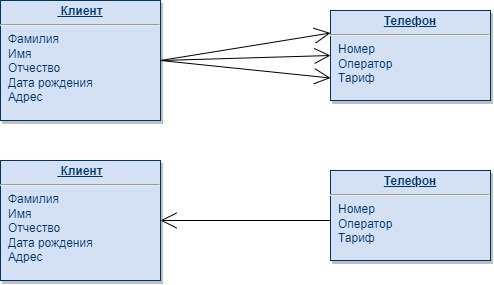
\includegraphics[scale = 0.5]{1/1kn.jpg}
    \caption{Связь один ко многим}
    \label{fig:onekn}
\end{figure}

\begin{figure}[!h]
    \centering
    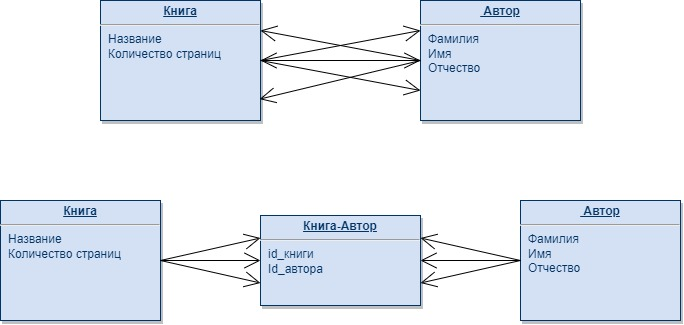
\includegraphics[scale = 0.5]{1/nkn.jpg}
    \caption{Связь многие ко многим}
    \label{fig:nkn}
\end{figure}


\begin{center}
\textit{\underline{Целостность данных.}}
\end{center}

Для пользователей важно, чтобы база данных отображала предметную область однозначно и непротиворечиво, т.е. чтобы она удовлетворяла условию целостности.

В теории баз данных под целостностью понимают свойство соответствия структуры и содержания базы данных предметной области. В реляционной модели данных определяются два основных требования, при которых обеспечивается целостность данных: \textbf{целостность сущностей} и \textbf{целостность ссылок.}

Каждый объект или наблюдение представляется в реляционной базе как группа взаимосвязанных элементов данных — кортеж некоторого отношения.

\textit{Требование целостности сущностей} заключается в том, чтобы каждый кортеж любого отношения отличался от другого кортежа этого отношения (т.е. любое отношение должно обладать первичным ключом).

\textit{Требование ссылочной целостности} состоит в том, что для каждого значения внешнего ключа, появляющегося в дочернем отношении, в родительском должен найтись кортеж с таким же значением первичного ключа.

Дополнительно по этой теме полезно почитать про нотацию "Воронья лапка" и ER модели: \url{https://clck.ru/q2Wet}


\newpage
\section{Билет 2. Операции над данными. Объединение, пересечение и разность. Произведение и соединение по условию. Деление. Ограничение, проекция и переименование. Реляционное исчисление.}

Два отношения называются  \textbf{совместимыми по типу}, если каждое из них имеет одинаковое множество имен атрибутов и если соответствующие атрибуты определены на одном и том же домене. 
(Домен атрибута — множество допустимых значений, которые может принимать атрибут). 

\textit{Замечание:} никакие реляционные операторы не передают результатирующему отношению никаких данных о потенциальных ключах.

\begin{enumerate}
    \item   \textbf{Объединением} двух совместимых по типу отношений A и B называется отношение с тем же заголовком, что и у отношений A и B, и телом, состоящим из кортежей, принадлежащих или A, или B, или обоим отношениям.

Синтаксис операции объединения: A UNION B


\textit{Замечание}: Объединение, как и любое отношение, не может содержать одинаковых кортежей. Поэтому, если некоторый кортеж входит и в отношение A, и отношение B, то в объединение он входит один раз.


\item 
\textbf{Пересечением} двух совместимых по типу отношений A и B называется отношение с тем же заголовком, что и у отношений A и B, и телом, состоящим из кортежей, принадлежащих одновременно обоим отношениям A и B.

Синтаксис операции пересечения: A INTERSECT B

\item  \textbf{Вычитанием (или разностью)} двух совместимых по типу отношений A и B называется отношение с тем же заголовком, что и у отношений A и B, и телом, состоящим из кортежей, принадлежащих отношению A и не принадлежащих отношению B. 

Синтаксис операции вычитания: A MINUS B

\item \textbf{Декартовым произведением} двух отношений $A(A_1, ..., A_n)$ и $B(B_1,..., B_m)$ называется отношение, заголовок которого является сцеплением заголовков отношений A и B: $(A_1, ..., A_n, B_1,..., B_m)$,
а тело состоит из кортежей, являющихся сцеплением кортежей отношений A и B: $(a_1, ..., a_n, b_1,..., b_m)$ таких, что $(a_1, ..., a_n) \in A, (b_1,..., b_m) \in B$

Синтаксис операции произведения: A TIMES В

\item    \textbf{Соединением} отношений A и B по условию c называется отношение (A TIMES B) WHERE c, где c представляет собой логическое выражение, в которое могут входить атрибуты отношений А и B и (или) скалярные выражения.

Таким образом, операция соединения есть результат последовательного применения операций декартового произведения и выборки. 


\item Пусть даны отношения $A(X_1, .., X_n, Y_1, ..., Y_m)$  $B(Y_1, ..., Y_m)$, причем атрибуты $Y_1, ..., Y_m$ - общие для двух отношений. \textbf{Делением} отношений A на B называется отношение с заголовком  $X_1, .., X_n$ и телом, содержащим множество кортежей $(x_1, .., x_n)$ таких, что для всех кортежей $(y_1, .., y_m) \in B$ в отношении A найдется кортеж $(x_1, .., x_n, y_1, .., y_m)$.

Отношение A выступает в роли делимого, отношение B выступает в роли делителя. Деление отношений аналогично делению чисел с остатком.

Синтаксис операции деления: A DEVIDBY B


\item  \textbf{Выборка (или ограничение)} возвращает отношение, содержащее кортежи из заданного отношения, которые удовлетворяют указанным условиям;

Синтаксис операции выборки: A WHERE c, c - условие 

\item \textbf{Проекцией} отношения A по атрибутам X, Y, ..., Z, где каждый из атрибутов принадлежит отношению A, называется отношение с заголовком (X, Y, ..., Z)  и телом, содержащим множество кортежей вида (x, y, ..., z) таких, для которых в отношении A найдутся кортежи со значением атрибута X равным x, значением атрибута Y равным y, …, значением атрибута Z равным z. 

Синтаксис операции проекции: A[X, Y, .., Z]

\item Операция \textbf{переименования} производит отношение, тело которого совпадает с телом операнда, но имена атрибутов изменены. 

Cинтаксис: R RENAME Atr1, Atr1, ... AS NewAtr1, NewAtr2, ..; где R - отношение, Atr1, Atr2.. - исходные имена атрибутов, NewAtr1, NewAtr2.. - новые имена атрибутов.

\end{enumerate}

\textbf{Реляционное исчисление} — декларативный язык для работы с отношениями, описывающий какими свойствами должен обладать требуемый результат.

\newpage
\section {Билет 3. Нормальные формы.}

Возможно полезно почитать и посмотреть примеры тут:

\url{https://habr.com/ru/post/254773/} 

\url{https://info-comp.ru/database-normalization}

\textbf{Нормальная форма} — требование, предъявляемое к структуре таблиц в теории реляционных баз данных для устранения из базы избыточных функциональных зависимостей между атрибутами (полями таблиц).

Цель нормализации: исключить избыточное дублирование данных, которое является причиной аномалий, возникших при добавлении, редактировании и удалении кортежей(строк таблицы).

3.1 \textbf{Первая нормальная форма}
Таким образом, чтобы база данных находилась в 1 нормальной форме, необходимо чтобы ее таблицы соблюдали следующие реляционные принципы:

\begin{itemize}
	\item В таблице не должно быть дублирующих строк
	\item В каждой ячейке таблицы хранится атомарное значение (одно не составное значение)
	\item В столбце хранятся данные одного типа
	\item Отсутствуют массивы и списки в любом виде
\end{itemize}

3.2 \textbf{Вторая нормальная форма}

Чтобы база данных находилась во второй нормальной форме (2NF), необходимо чтобы ее таблицы удовлетворяли следующим требованиям:

\begin{itemize}
	\item Таблица должна находиться в 1НФ
	\item Таблица должна иметь первичный ключ
	\item Все неключевые столбцы таблицы должны зависеть от полного ключа (в случае если он составной)
\end{itemize}

Если ключ составной, т.е. состоит из нескольких столбцов, то все остальные неключевые столбцы должны зависеть от всего ключа, т.е. от всех столбцов в этом ключе. Если какой-то атрибут (столбец) зависит только от одного столбца в ключе, значит, база данных не находится во второй нормальной форме.

3.3 \textbf{Третья нормальная форма}

Требование третьей нормальной формы (3NF) заключается в том, чтобы в таблицах отсутствовала транзитивная зависимость.

Транзитивная зависимость – это когда неключевые столбцы зависят от значений других неключевых столбцов.

\textbf{Нормальная форма Бойса-Кодда (НФБК)} (частная форма третьей нормальной формы)

\begin{itemize}
	\item Таблица должна находиться в 3НФ. 
	\item Ключевые атрибуты составного ключа не должны зависеть от неключевых атрибутов.
\end{itemize}

\color{blue} !!Есть вероятность, что дальше не нужно, так как на 2 семинаре модель бд мы проверяли до этого места (записи 1-ого семинара нет, так что проверить не могу)

В по этой теме полезно почитать про нотацию "Воронья лапка" и ER диаграммы
\color{black} 

3.4 \textbf{Четвертая нормальная форма}
Таблица должна находиться в НФБК.
Требование четвертой нормальной формы (4NF) заключается в том, чтобы в таблицах отсутствовали нетривиальные многозначные зависимости.

В таблицах многозначная зависимость выглядит следующим образом.

Начнем с того, что таблица должна иметь как минимум три столбца, допустим A, B и C, при этом B и C между собой никак не связаны и не зависят друг от друга, но по отдельности зависят от A, и для каждого значения A есть множество значений B, а также множество значений C.

В данном случае многозначная зависимость обозначается вот так:

A —> B

A —> C

Если подобная многозначная зависимость есть в таблице, то она не соответствует четвертой нормальной форме.

3.5 \textbf{Пятая нормальная форма}

Отношения находятся в 5НФ, если оно находится в 4НФ и отсутствуют сложные зависимые соединения между атрибутами.

Если «Атрибут1» зависит от «Атрибута2», а «Атрибут2» в свою очередь зависит от «Атрибута3», а «Атрибут3» зависит от «Атрибута1», то все три атрибута обязательно входят в один кортеж.

Это очень жесткое требование, которое можно выполнить лишь при дополнительных условиях. На практике трудно найти пример реализации этого требования в чистом виде.

\textit{Пояснение:} Например, некоторая таблица содержит три атрибута «Поставщик», «Товар» и «Покупатель». Покупатель1 приобретает несколько Товаров у Поставщика1. Покупатель1 приобрел новый Товар у Поставщика2. Тогда в силу изложенного выше требования Поставщик1 обязан поставлять Покупателю1 тот же самый новый Товар, а Поставщик2 должен поставлять Покупателю1, кроме нового Товара, всю номенклатуру Товаров Поставщика1. Этого на практике не бывает. Покупатель свободен в своем выборе товаров. Поэтому для устранения отмеченного затруднения все три атрибута разносят по разным отношениям (таблицам). После выделения трех новых отношений (Поставщик, Товар и Покупатель) необходимо помнить, что при извлечении информации (например, о покупателях и товарах) необходимо в запросе соединить все три отношения. Любая комбинация соединения двух отношений из трех неминуемо приведет к извлечению неверной (некорректной) информации. Некоторые СУБД снабжены специальными механизмами, устраняющими извлечение недостоверной информации. Тем не менее, следует придерживаться общей рекомендации: структуру базы данных строить таким образом, чтобы избежать применения 4НФ и 5НФ.



\textbf{Доменно-ключевая нормальная форма}

Ограничение домена – это ограничение, предписывающее использование для определенного атрибута значений только из некоторого заданного домена (набора значений).

Ограничение ключа – это ограничение, утверждающее, что некоторый атрибут или комбинация атрибутов представляет собой потенциальный ключ.

Таким образом, требование доменно-ключевой нормальной формы заключается в том, чтобы каждое наложенное ограничение на таблицу являлось логическим следствием ограничений доменов и ограничений ключей, которые накладываются на данную таблицу.

Таблица, находящаяся в доменно-ключевой нормальной форме, обязательно находится в 5NF. Однако, стоит отметить, что не всегда возможно привести таблицу к доменно-ключевой нормальной форме, более того, не всегда возможно получить ответ на вопрос о том, когда может быть выполнено такое приведение.

\textbf{Шестая нормальная форма}

Переменная отношения находится в шестой нормальной форме тогда и только тогда, когда она удовлетворяет всем нетривиальным зависимостям соединения. Из определения следует, что переменная находится в 6НФ тогда и только тогда, когда она неприводима, то есть не может быть подвергнута дальнейшей декомпозиции без потерь. Каждая переменная отношения, которая находится в 6НФ, также находится и в 5НФ.

Идея «декомпозиции до конца» выдвигалась до начала исследований в области хронологических данных, но не нашла поддержки.
\newpage
\section {Билет 4. Индексы (дерево, карты, хэш).}

Индекс применяется для ускорения поиска нужных строк (в операциях
выборки/обновления/удаления). Индекс является упорядоченной структурой (записи в индексе хранятся в отсортированном виде). После создания индекса в актуальном состояние его поддерживает СУБД.

По умолчанию команда CREATE INDEX создаёт индексы-B-деревья, эффективные в большинстве случаев. Выбрать другой тип можно, написав название типа индекса после ключевого слова USING. 

\textbf{B-дерева:} 

Структура B-дерева: 
\begin{itemize}
    \item При построении B-дерева применяется фактор t, который называется минимальной степенью. Каждый узел, кроме корневого, должен иметь, как минимум t – 1, и не более 2t – 1 ключей. Обозначается n[x] – количество ключей в узле x.
    \item Ключи в узле хранятся в неубывающем порядке. Если x не является листом, то он имеет n[x] + 1 детей. Если занумеровать ключи в узле x, как k[i], а детей c[i], то для любого ключа в поддереве с корнем c[i] (пусть k1), выполняется следующее неравенство $-k[i-1] \leq k1 \leq k[i]$ (для $c[0]: k[i-1] = -\infty,$ а для $c[n[x]]: k[i] = +\infty)$. Таким образом, ключи узла задают диапазон для ключей их детей.
    \item Все листья B-дерева должны быть расположены на одной высоте, которая и является высотой дерева. Высота B-дерева с $n \geq 1$ узлами и минимальной степенью $t\geq 2$ не превышает logt(n+1).
\end{itemize}

На рисунке \ref{fig:tree} изображен пример B-дерева. 

\begin{figure}[!h]
    \centering
    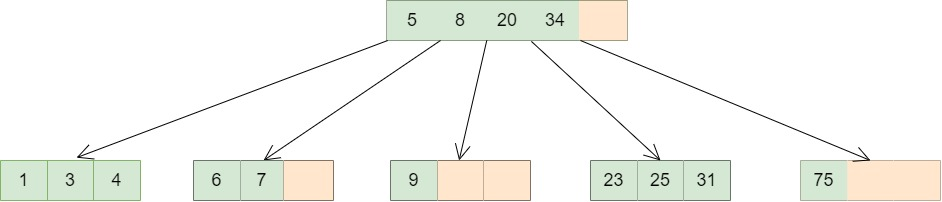
\includegraphics[scale = 0.5]{4/tree.jpg}
    \caption{Пример B-дерева}
    \label{fig:tree}
\end{figure}


B-деревья могут работать в условиях на равенство и в проверках диапазонов с данными, которые можно отсортировать в некотором порядке. Точнее, планировщик запросов PostgreSQL может задействовать индекс-B-дерево, когда индексируемый столбец участвует в сравнении 

\textit{Недостатки}: поиск только по одному столбцу. (Если нам нужно найти брюнетов с зелеными глазами, то по дереву мы найдем брюнетов, а дальше уже придется проверять их всех, то есть не использовать индексы)

\textbf{Bitmap(карты)} 

В bitmap-структурах создается двухмерный массив со столбцом для каждой строки в индексируемой таблице. Каждый столбец представляет отдельное значение в bitmap-индексе. Этот двухмерный массив показывает каждое значение индекса, умноженное на количество строк в этой таблице.

Идея поиска по такому индексу предсавленна на рисунке \ref{fig:Map}  

\begin{figure}[!h]
    \centering
    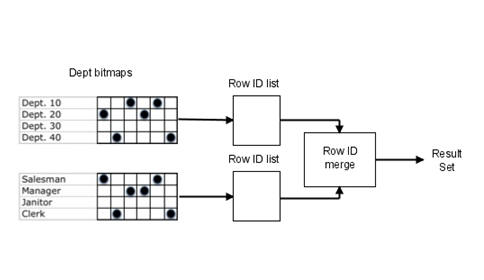
\includegraphics[scale = 0.3]{4/Map.jpeg}
    \caption{Пример поиска по индексу}
    \label{fig:Map}
\end{figure}


Берем строчку из первого индекса (по нашим условиям), и строчку из второго индекса. Дальше логические операции заменяем на побитовые и проводим их на наших выбранных строчках (Рис.\ref{fig:BMap}).

\begin{figure}[!h]
    \centering
    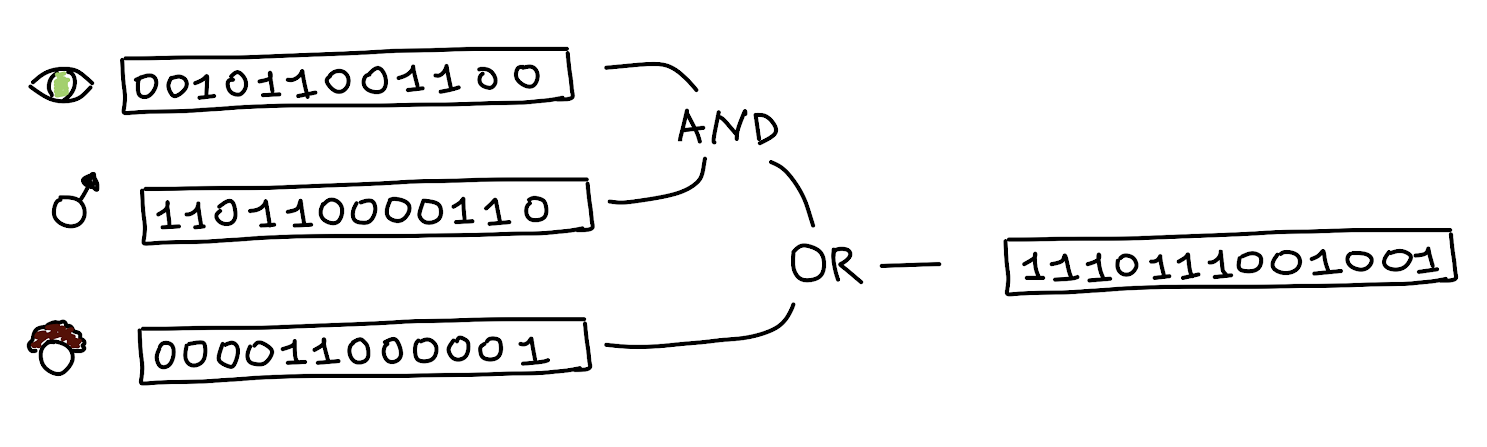
\includegraphics[scale = 0.3]{4/BitMat.png}
    \label{fig:BMap}
    \caption{Пример поиска по индексу}
\end{figure}

\textit{Недостатки:} Предположим, мы заблокировали запись -> нужно заблокировать часть индекса, где она учавствует (в дереве - только лист, там мало значений: k), а вот у карты нужно блокировать всю строку индекса - это много.


\textbf{Хеш - индексы} 
Хэш-индекс (Hash Index) основан на хэш-таблице, он полезен только для точного поиска по каждому столбцу в индексе. Просто по значениям в таблице вычисляем некоторую хеш функцию и значения таблицы помещаем в ячейку с номером хеша. 


\newpage
\section {Билет 5. Оптимизация запросов, построение и оценка планов запросов.}

Операции существуют 2-ух типов: 
\begin{itemize}
    \item DML - это аббревиатура от языка манипулирования данными. Он используется для извлечения, хранения, изменения, удаления, вставки и обновления данных в базе данных.

Примеры: операторы SELECT, UPDATE, INSERT, DELETE, MERGE

\item DDL - это аббревиатура языка определения данных. Он используется для создания и изменения структуры объектов базы данных.

Примеры: операторы CREATE, ALTER, DROP
\end{itemize}

Приведем синтаксис оператора SELECT: 

SELECT поля

FROM таблица 

WHERE условия 

С оператором SELECT дополнительно можно применять GROUP BY и HAVING.  
\\[10pt]

\begin{enumerate}
    \item \textbf{Способы соединения таблиц }

Хотим понять каким способом делать соединения таблиц. Пусть хотим соединить 2 таблицы по id, те по A.id = B.id с условием A.a = x, B.b = y.

\textit{Способ 1}: \textbf{nested loop (вложенный цикл)}

Выбрать все данные из одной таблицы (например А по условию A.a= x) после этого для каждого id выбрать все подходящие из B (по индексу и значению B.b = y). По фатку это 2 цикла вложенных в друг друга.

Сложность: $N^2$. Если критерий x является очень хороший, то сложность становиться N. 

\textit{Способ 2}: \textbf{merge join (слияние)}

Взять наши данные и отфильтровать отдельно по условию x в таблице А, по условию y в таблице В, а дальше отсортировать и после этого соединить два отсортированных массива.

Сложность: $NLogN$. Если критерий x является очень хороший, а таблица В большая, то сложность останется такой же. 

Из-за этого нельзя сказать, какой способ (1 или 2) лучше. 

\textit{Способ 3}: \textbf{hash join (хеширование)}

При соединении хешированием строки одного набора помещаются в
хеш-таблицу, содержащуюся в памяти, а строки из второго набора
перебираются, и для каждой из них проверяется наличие
соответствующих строк в хеш-таблице.

Ключом хеш-таблицы является тот столбец, по которому выполняется
соединение наборов строк.

Такой способ эффективен для больших выборок. 

\item  \textbf{Способы доступа к данным таблицы}

Теперь мы хотим выполнять запросы к одной таблице. У нас остается A.a= x. 

\textit{Способ 1}: \textbf{full scan} - проходит таблицу целиком. 

\textit{Способ 2}: \textbf{index} - используем индекс, если нужное значение заиндексировано и мы ищем какой-то диапазон. 

Пример: номер зачетки заиндексирован, и мы просто хотим найти номер зачетки, который равен x или находится в каком-то диапазоне. 

\textit{Способ 3}: \textbf{index scan} - предположим, что значение заиндексировано, а мы, например, хотим выбирать по значениям какой-то функции от значения в таблице, сам индекс такого не даст. Так что нам придется в любом случае читать данные. Вся запись весит много, а вот индекс, который хранит данные только одного значения, по факту весит гораздо меньше. 

Был пример с зачетками: заиндексирован номер зачетки, хотим получить человека с номером зачетки таким, что Sin от номера зачетки лежит в [0.5, 0.6], сам индекс такого не даст. Индекс хранит только номера зачеток, а полная запись содержит ФИО, место рождения, дату рождения и еще много всего. Соответственно, занимает много памяти и времени, если все читать из памяти для поиска, а в индексе мы читаем только номер зачетки, что весит гораздо меньше -> быстрее. 


\end{enumerate}


Пусть у нас есть запрос, в котором присутсвуют таблицы A, B, C, D. Нужно построить план выполнения запроса, которые выглядит как дерево (Рис. \ref{fig:plan1}). Стоит помнить, что это не синтаксический разбор. Тут мы решили отсканировать A full scan, B по индексу, а потом сделать между ними hash join. 

\begin{figure}[h!]
    \centering
    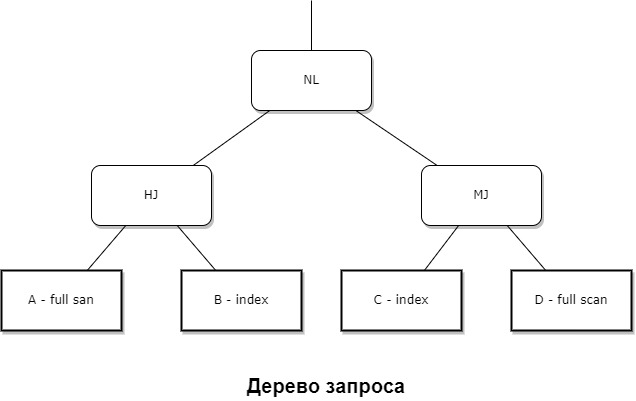
\includegraphics[scale = 0.5]{5/plan.jpg}
    \caption{}
    \label{fig:plan1}
\end{figure}

Скорость выполнения ОЧЕНЬ сильно зависит от оптимальности плана запроса.
\\[20pt]
Для выбора плана запроса в базе данных сущестсвует \textbf{оптимизатор}. Он получает на вход разобранный синтаксически SELECT и выдает план выполнения запроса (внутри оптимизатора еще проверяются права доступа). 

\textbf{Виды оптимизаторов:} 
\begin{itemize}
    \item \textbf{Rule (cинтаксический)}. Основан на словарях, для того, чтобы выбрать лучший план запроса просматривает все условия, которые фигурируют в запросе и проводит анализ без учета данных (только на объялении структуры). Например в нем прошито правило, что индексный поиск по уникальному индексу - наилучший, после него идет не уникальный индекс, потом index scan, а потом full scan. Правил около 15, но суть одна (по факту прописаны приоритеты). Работает это очень быстро, но наилучший план он выбрать не может.
    
Почему плохой оптимизатор: мы хотим найти в базе студентов Иванова Рамиля, тогда нам выгодно в первую очередь искать по имени, так как Ивановых скорее всего много. Этот оптимизатор такое не учитывает. 

\item \textbf{Cost}. Такой вид оптимизатора строит много планов выполнения запроса и считает их стоимость. По факту делает "виртуальное" выполнение запроса. У него есть оценки сколько понадобится сделать действий, чтобы произвести какой-либо способ доступа. 
    
Например, если в оптимизаторе есть информация, что в таблице 1к блоков и в ней 1 миллион записей при этом уникальных 100к, тогда full scan должен прочитать все блоки и выбрать где-то 10 записей. Если же будет использоваться индекс, то нужно будет прочитать 10 блоков и выбрать 10 записей. 
    
Так для каждого плана появляется цена выполнения. Рассмотрим модель работы Oracle DB: при расчете стоимости все операции (чтение диска, стоимость сортировки, процессорное время...) конвертируются в некоторую условную 'валюту', которая называется \textbf{логическим чтением блоков}. Стоимость высчитывается в этой валюте. Часто планы запроса хранятся, чтобы не пересчитываться много раз. 
    
Сложности: 
    
1) количество вариантов возможных планов запросов. Из-за этого оптимизатор работает классическими алгоритмами частичного обхода дерева (основная идея: берутся наилучшие ветки, начинаем спуск, если ветка оказалась плохой, то мы ее откидываем и дальше не проверяем). И еще можно поставить ограничение на количество вариантов. 
    
2) Где брать данные, чтобы понимать, сколько мы получим записей после какой-то выборки. Если мы выбираем по фиксированным условиям (имя = Петр), то помогает построение гистограмм: по каждому столбцу строим общие характеристики и строим гистограммы, сколько значений попадают в какой-то диапазон (на букву П у нас 8млн записей, на букву К 10млн и тд). Это частично решает проблему (так как строить уникальные гистограммы слишком затратно). 
    
Статистика не работает, если мы используем ограничения, которые невозможно заранее просчитать. Таких бывает 3 вида: 
\begin{enumerate}
    \item Для столбцов, которые имеют близкие значения с очень разными частотами.
    \item Использование ограничений, которые содержат функцию (хотим выбрать студентов у которых третий знак после запятой в синусе от веса студента равен 3, понятно, что гистограмма бесполезна).
    \item (самый важный для нас) Если мы имеем дело с доступом к удаленным данным: получаем данные с другого сервера, но статистики его мы не знаем.
\end{enumerate}

Есть два подхода к решению таких сложностей: 

\begin{enumerate}
    \item Семплирование - получение примера данных. (Например в Oracle DB: A SAMPLE (5) - хотим считать из таблицы 5\% случайных блоков). Берутся примеры данных из всех таблиц, и на них проверяются условия выборки. Потом расширяем полученные данные на всю таблицу и считаем, что получили всю статистику (для удаленных данных просто просим прислать какой-то процент блоков и далее аналогично). Способ хороший так как дает +- точные результаты, но есть недостаток - стоимость подготовки плана (может присылаться очень много данных).
    \item Перестраивание дерева на ходу. Реализуется сложно, но принцип простой:  смотрим на картинку плана запроса. Мы предполагаем, что при объединении HJ А и В мы получим примерно 4 записи (не стоимость) и тогда выше стоящий NL - оптимальный вариант. Начали выполнять, в момент соединения А и В HJ мы получили 400к записей и в таком случае система останавливает выполнение запроса и производит пересчет частей, которые мы еще не выполнили.
\end{enumerate}
\end{itemize}

Существует еще один метод оптимизации запроса - \textbf{переписывание}. 

Вспоминаем три структуры данных: 

\begin{enumerate}
    \item \textit{таблицы} - просто хранят данные;
    \item  \textit{представления} - хранят запросы к таблицам (возможно, в виде плана запроса);
    \item \textit{материальные представления (мп)} - хранят результат выполнения какого-то запроса. 
\end{enumerate}

Нас интересуют материальные представения. У мп есть метка вычисления (мы можем сказать, когда менялись таблицы и когда было посчитано материальное представление). Смотрим на рисунок плана (Рис. \ref{fig:plan1}). Пусть мы захотели отдельно посмотреть HJ для A и В. Если HJ был сделан после изменения таблиц, то мы можем удалить часть дерева ниже HJ и подставить туда материальное представление (Рис. \ref{fig:plan2}). Так мы сокращаем размер вычислений.  

 \begin{figure}[h!]
     \centering
     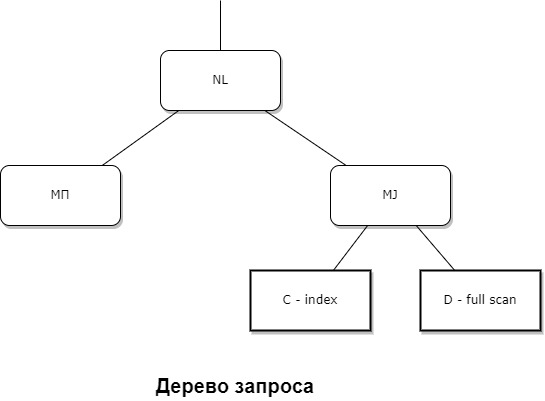
\includegraphics[scale = 0.5]{5/plan2.jpg}
     \caption{После добавления МП}
     \label{fig:plan2}
 \end{figure}

Механизмы получения данных из внешней системы (терминология  Oracle DB)
\begin{itemize}
    \item  dblink -  связывают бд одного типа (умеют все делать так как все друг о друге знают);
    \item внешние таблицы - если надо подключить статические данные (например csv файл). Может быть медленным, особо ничего нет;
    \item шлюзы (ODBC).
\end{itemize}

\newpage
\section {Билет 6. Транзакции, блокировки, версионность.}


\textbf{Транзакция} — это набор операций в базе данных, которые должны быть либо все выполнены, либо все не выполнены. Транзакции применяются для обеспечения безопасности, верности и непротиворечивости данных в таблице.

\textbf{1 Феномен грязной записи}

Пример: Транзакция T1 модифицирует элемент данных. После этого другая транзакция T2 тоже модифицирует этот элемент данных перед тем, как T1 выполнит COMMITT или ROLLBACK. Если T1 или T2 после этого выполнит ROLLBACK, то становится непонятным, каким должно быть корректное значение элемента.

\textbf{2 Феномен «грязного» чтения (dirty read)}

Транзакция T1 модифицировала содержимое элемента данных. После этого другая транзакция T2 прочитала содержимое этого элемента данных, до того как транзакция T1 выполнила операцию COMMIT (зафиксировалась) или ROLLBACK (откатилась). Если T1 завершается операцией ROLLBACK, то получается, что транзакция T2 прочитала реально не существующие данные.


\textbf{2.5 Феномен потерянной модификации}

Аномалия потерянной модификации происходит в случае, когда транзакция T1 прочитала элементы данных, после нее T2 их модифицировала (возможно, исходя из предыдущего чтения), после чего T1 (основываясь на ранее прочитанном ею значении) модифицирует содержимое элемента данных и фиксируется.

\textbf{3 Феномен неповторяемого чтения (unrepeatable read)}

Транзакция T1 прочитала содержимое элемента данных. После этого другая транзакция T2 модифицирует или удаляет этот элемент данных и фиксируется. Если T1 после этого попытается прочитать содержимое этого элемента данных снова (она еще не завершилась), то она получит другое значение или обнаружит, что элемент данных больше не существует.

\textbf{4 Феномен фантомов}

Транзакция T1 прочитала содержимое нескольких элементов данных, удовлетворяющих некоторому предикату . После этого транзакция T2 создает элемент данных, удовлетворяющий этому предикату, и фиксируется. Если транзакция T1 повторит чтение с тем же предикатом , то получит уже другой набор данных, отличный от полученного в первый раз.

Первый способ решения феноменов - \textbf{блокировки}: запрещается доступ к строкам (а может и ко всей таблице) по определенным условиям. Блокировки бывают длинные (до конца транзакций) и короткие (на время выполнения операции). Блокировки на несколько операций не выставляются. 

В таблице показано какие блокировки решают феномены:

\begin{center}
	\begin{tabular}{c|c c}
		Феномен & Чтение & Запись \\
		1 & - & Д \\
		2 & К & Д\\
		3 & Д на курсор & Д \\
		4 & Д на предикат & Д\\
	\end{tabular}
\end{center}

Можно было бы выбрать 3 уровень и радоваться, но нет - будет очень многозаблокированных данных. Блокировки уже мало где используются. 

\textbf{Версионность.} 

Мы продолжаем выставлять блокировки на запись, но при чтении мы не блокируем запись, а запоминаем в какой момент произвели чтение. 

Пусть есть блок b и ему прписано время 1. В момент времени 1 мы начали выполнять SELECT, который когда-нибудь дойдет до блока b. В момент времени 2 мы переписали значение блока b. Тогда данные перезаписываются, b приписывается время 2, а часть блока уезжает в сегмент отката. Когда транзакция доходит до блока b, она видит, что у него время 2 (позже ее начала) и мдет в сегмент отката за нужными записями. 

\begin{figure}[H]
	\centering
	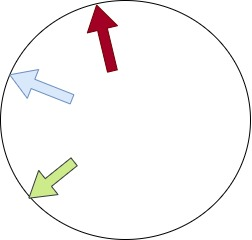
\includegraphics[scale = 0.5]{6/vers.jpg}
	\label{fig:vers}
	\caption{Сегмент отката}
	
\end{figure}

На рисунке \ref{fig:vers} изображена структура сегмента отката. Голубым изображен хвост, а зеленым голова. Голова начинает догонять свой хвост. Но когда мы говорим COMMIT мы передвигаем хвост на последнюю незакоммиченную транзакцию. Если хвост указывет на временную метку 4, голова на 10, а наш запрос пытается получить данные за первый (1) момент времени (показано красной стрелочкой), то произойдет ошибка (снимок слишком старый). Если голова дойдет до хвоста, то будет фатальная ошибка у всех пользователей. 


Журнал версионности также служит способом восстановления бд. Если писать изменения данных сразу на диск, то бд будет рабоатать супер долго. Просто в памяти хранить нельзя (можем потерять все изменения даже если были коммиты). Однако, можно писать на диск сегмент отката. Туда пишутся только сами изменения (это весит гораздо меньше) и мы говорим пользователю, что все сохранили, только если сегмент отката записался на диск. 

\textbf{Простейший пример взаимной блокировки (deadlock):}

\begin{center}
	\begin{tabular}{c|c | c}
		Шаг	& Процесс 1	& Процесс 2 \\
		0	&Хочет захватить A и B, начинает с A &	Хочет захватить A и B, начинает с B \\
		1&	Захватывает ресурс A &	Захватывает ресурс B \\
		2&	Ожидает освобождения ресурса B	& Ожидает освобождения ресурса A \\
		3	&Взаимная блокировка & Взаимная блокировка
	\end{tabular}
\end{center}

Для решения просто кого-то вышибают. Сложнее обнаружить такую ситуацию, для этого используют посик циклов в графе. Пример цикла на Рис.\ref{fig:dead}. R - ресурс. P - процесс. 

\begin{figure}[H]
	\centering
	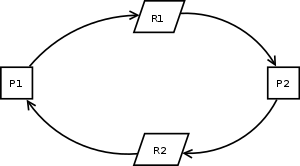
\includegraphics[scale = 0.5]{6/deadlock.png}
	\label{fig:dead}
	\caption{Граф deadlock}
	
\end{figure}
\newpage
\section {Билет 7. Распределенные запросы. Распределенные и кластерные базы данных. Распределенные транзакции.}

Мы можем использовать сервер баз данных, чтобы запрашивать и обновлять несколько баз данных на нескольких серверах одного и того же экземпляра. Запросы такого типа называются \textbf{распределенными запросами}. Этот термин не ограничивается операторами SELECT и часто используется для более общего обозначения любой операции DML (Data Manipulation Language) или выполнения подпрограммы, которая возвращает объекты или ссылается на объекты вне локальной базы данных.
В распределенных запросах для разных серверов серверы баз данных могут находиться на одном хост-компьютере, в одной и той же сети или на шлюзе.

\bigskip
\textbf{Распределённая база данных} - это такая база данных, составные части которой размещаются в различных узлах компьютерной сети в соответствии с каким-либо критерием.

Распределённая база данных — это именно единая база данных, а не произвольный набор файлов, индивидуально хранимых на разных узлах сети и являющейся распределенной файловой системой. Данные представляют собой РБД, только если они связаны в соответствии с некоторым структурным формализмом, реляционной моделью, а доступ к ним обеспечивается единым высокоуровневым интерфейсом.

Распределённые базы могут иметь разный уровень реплицированности — от полного отсутствия дублирования информации, до полного дублирования всей информации во всех распределённых копиях (например, блокчейн).

Распределение (включая фрагментацию и репликацию) базы данных по множеству узлов невидимо для пользователей. Это свойство называется прозрачностью, а технология распределения и реплицирования данных по множеству компьютеров, связанных сетью, является основополагающей для реализации концепции независимости данных от среды хранения. Это обеспечивается за счёт нескольких видов прозрачности:

\begin{enumerate}
	\item[\textbullet] прозрачность сети, а следовательно, прозрачность распределения
	\item[\textbullet] прозрачность репликации
	\item[\textbullet] прозрачность фрагментации
	\item[\textbullet] прозрачность доступа, означающая, что пользователи имеют дело с единым логическим образом базы данных и осуществляют доступ к распределенным данным точно так же, как если бы они хранились централизованно.
\end{enumerate}

В идеале полная прозрачность подразумевает наличие языка запросов к распределённой СУБД, не отличающегося от языка для централизованной СУБД.

\bigskip
Основными структурами построения кластерных баз данных являются:
\begin{enumerate}
	\item \textbf{Shared Disk (SD)} - случай, когда база данных, располагающаяся на нескольких компьютерах, использует одни и те же устройства хранения.
	
	\item \textbf{Shared Memory (SM)} - случай, когда много процессоров в базе данных, возможно, расположенных на разных машинах, используют общую (разделяемую) память.
	
	\item \textbf{Shared Nothing (SN)} - случай, когда ни устройства хранения, ни память систем не разделяются. В таких системах каждый узел обслуживает свой фрагмент базы данных, уникальность которого обеспечивается либо организацией базы данных, либо дополнительными средствами управления и мониторинга СУБД.
	
	\item \textbf{Shared Everything (SE)} - случай симбиоза SM+SD, когда СУБД использует и общие устройства ввода-вывода, и память. К таким системам относится, например, Oracle RAC.
\end{enumerate}

\begin{figure}[h]
	\centering
	\begin{subfigure}[b]{0.2\textwidth}
		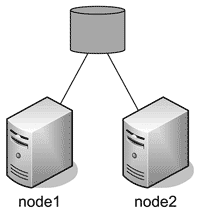
\includegraphics[width=\textwidth]{7/07_01.png}
		\caption{Shared Disk}
	\end{subfigure}
	\hfill
	\begin{subfigure}[b]{0.2\textwidth}
		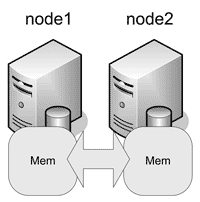
\includegraphics[width=\textwidth]{7/07_02.png}
		\caption{Shared Memory}
	\end{subfigure}
	\hfill
	\begin{subfigure}[b]{0.2\textwidth}
		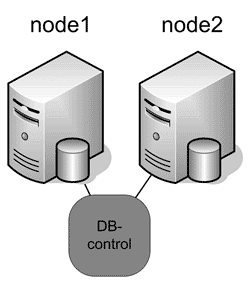
\includegraphics[width=\textwidth]{7/07_03.png}
		\caption{Shared Nothing}
	\end{subfigure}
	\hfill
	\begin{subfigure}[b]{0.2\textwidth}
		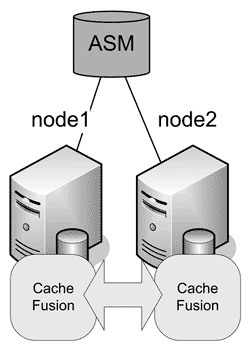
\includegraphics[width=\textwidth]{7/07_04.png}
		\caption{Shared Everything}
	\end{subfigure}
	
	\caption{Кластерные БД}
\end{figure}


\bigskip
\href{https://en.wikipedia.org/wiki/Distributed_transaction}{Распределенная транзакция} — это транзакция, затрагивающая несколько ресурсов. Для фиксации распределенной транзакции все участники должны гарантировать, что любое изменение данных будет постоянным. Изменения должны сохраняться даже в случае фатального сбоя системы или других непредвиденных событий. Если хоть один из участников не сможет предоставить такую гарантию, вся транзакция завершится с ошибкой и будет выполнен откат любых изменений данных внутри области транзакции.
\newpage
\section {Билет 8. Одно-, двух- и трехзвенные архитектуры.}

Основная архитектура приложения может принимать различные формы. Основные различия между архитектурами приложений состоят в количестве систем, участвующих в работе приложения. Эта классификация производится по количеству \textbf{звеньев (tiers)}.

Каждое приложение базы данных состоит из трех отдельных компонент:
\begin{enumerate}
	\item[\textbullet] Службы базы данных (database services). Это конечный сервер базы данных и данные, которые размещены в этой базе данных.
	\item[\textbullet] Службы приложения (application services). Это механизмы манипулирования данными, извлекаемыми из базы данных. Логика их работы определяется приложением или потребностями бизнеса.
	\item[\textbullet] Службы представления (presentation services). Это пользовательский интерфейс. Службы представления должны быть способными манипулировать данными таким образом, чтобы это было понятно пользователям.
\end{enumerate}

\begin{figure}[h]
	\centering
	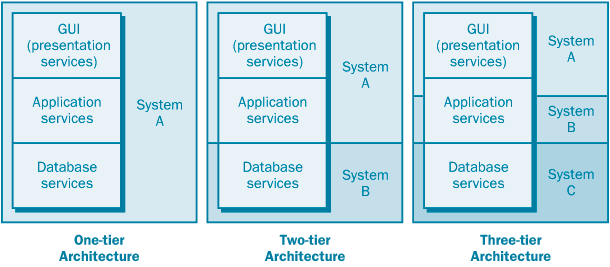
\includegraphics[scale=0.75]{8/08_01.png}
	\caption{Одно-, двух- и трехзвенные архитектуры}
	\label{fig:my_label5}
\end{figure}

Различие между однозвенной, двухзвенной и трехзвенной архитектурами зависит от того, каким образом разделяются на части эти компоненты. В однозвенной архитектуре они все являются частями одной программы. В двухзвенной архитектуре эти компоненты разделены на две отдельные части. В трехзвенной архитектуре компоненты разделены на три отдельные части.

\bigskip
Однозвенная архитектура – это система, в которой все службы базы данных, приложения и представления (пользовательский интерфейс) размещены на одной системе. Системы такого типа не производят обработку вне тех компьютеров, на которых они исполняются. Примером однозвенной архитектуры может служить база данных Microsoft Аccess с локальными службами представления.

\bigskip
В двухзвенных архитектурах службы представления и база данных размещаются на разных системах (компьютерах). Уровень служб представления (пользовательский интерфейс) обычно включает в себя логику работы приложения. Хорошим примером двухуровневого приложения является приложение, использующее SQL Server Enterprise Manager. У таких приложений пользовательский интерфейс и логика работы приложения размещаются в Enterprise Manager, но все данные, необходимые для функционирования приложения, находятся в базе данных SQL Server на другом компьютере.

\bigskip
В трехзвенных архитектурах уровень базы данных, уровень приложения и уровень служб представления выделены в три разные компоненты. В типичных трехзвенных приложениях используется промежуточный уровень для обслуживания многочисленных соединений от уровня служб представления, благодаря чему уменьшается количество соединений с SQL Server. Кроме того, этот промежуточный уровень может выполнять значительный объем работы, связанной с реализацией специфики целевых задач (логики предметной области), освобождая базу данных для решения тех задач, которые она выполняет лучше всего, – для доставки требуемых данных.

\bigskip
Фактически, обычно системы начинаются с одного сервера базы данных, соединенного с несколькими серверами приложений, которые, в свою очередь, обслуживают много компьютеров-клиентов. Решения, принимаемые при проектировании системы, зависят от количества ее пользователей и выбранного вами приложения.
\newpage
\section {Билет 9. IP, TCP, UDP, VPN, NAT}

\href{https://ru.wikipedia.org/wiki/IP}{IP} - специальный протокол,позволяющий осуществлять передачу сообщений между устройствами, находящимися в одной сети посредством идентификации этих устройств 4-байтовыми кодами (адресами).

Его работу можно полностью сравнить с работой Почты России. Если положить письмо в ящик, то оно \textbf{может быть} дойдёт до адресата. При этом, если положить 10 писем в ящик, то какое-то количество из них, наверняка, дойдёт, однако \textbf{неизвестно, в каком порядке}.

Естественно, в таких условиях программам работать было бы не комфортно, поэтому на базе протокола IP были придуманы более хитрые протоколы, про которые мы и поговорим далее.

\bigskip
\href{https://ru.wikipedia.org/wiki/UDP}{UDP} - протокол на базе IP-протокола, позволяющий обмениваться данными. Работает следующим образом: данные разбиваются на пакеты, которые по своему размеру подходят для передачи по IP-протоколу, и отправляет эти пакеты, пронумеровав их. На стороне адресата эти пакеты посредством нумерации собираются обратно в исходные данные.

UDP \textbf{не поддерживает} подтверждение о получении пакета, то есть, что-то, возможно, не дойдёт. Однако внутри одного пакета данных UDP гарантирует, что все данные дойдут в целостности (если они вообще дойдут).

Используется в основном в стриминговых передачах (например, онлайн-трансляция видео или аудио, передача показаний датчиков в реальном времени). Основная идея - в отличие от TCP, неважно, если какие-то данные не дошли. Ну будет пробел и будет (не показывать же вам не дошедшие кадры из фильма через 5 секунд, как вы уже этот момент просмотрели).

\bigskip
\href{https://ru.wikipedia.org/wiki/Transmission_Control_Protocol}{TCP} - более сложный протокол передачи данных. Всё так же режет данные на более мелкие пакеты и нумерует их, однако отправка более хитрая.

TCP имеет буфер (для пример скажем, длины 4, хотя в реальности он гораздо больше), в котором размещены пакеты данных. Он отправляет данные из буфера и (в отличие от UDP!) ждёт.

Когда адресат получает, скажем, пакет данных №3, он посылает подтверждение, что третий пакет получен и контрольная сумма сошлась. После этого TCP убирает из буфера пакет №3 и помещает туда следующий (в нашем примере, пакет №5). По мере того, как приходят подтверждения, пакеты из буфера убираются и заменяются на новые.

Если на пакет долго не было подтверждения, то он отправляется ещё раз. Передача завершается только тогда, когда на все пакеты пришло подтверждение. Таким образом, можно гарантировать целостность передачи всего набора данных (или узнать, какие именно пакеты не дошли).

TPC применяется, например, при передаче файлов или просто каких-то данных в реляционных системах.

\bigskip
При передаче данных возникает вопрос, насколько мелко стоит делить их на пакеты. Ведь при ошибке, скажем, 1 раз в 1000 байт, если делить данные на пакеты по 100 байт, ошибка будет в среднем в 1 из 10 пакетов (то есть, в среднем, повторно пересылать придётся около 10\% данных). А если делить на пакеты по 500 байт, то ошибка будет в каждом втором пакете.

С одной стороны, общий принцип пересылки - чем меньше пакет, тем больше вероятность, что он дойдёт. 

С другой стороны, в случае TCP-протокола, больше пакетов = больше ответных подтверждений, что будет забивать канал обратной связи. К тому же, не стоит забывать, что каждый пакет имеет заголовок (информация о том, кто отправитель, кто адресат, номер пакета, контрольная сумма и т.д.) фиксированного размера, не зависящего от разбиения. Поэтому, если размер заголовка, скажем, 100 байт, при разбиении данных на пакеты по 500 байт, итоговый размер пересланных данных вырастет на $\frac{1}{5}$. А если делить на пакеты по 100 байт, то итоговый размер пересылки вырастет в 2 раза.

\textbf{Мораль проста надо делить данные на как можно бОльшие пакеты.}

Одной отличительной чертой TCP является то, что он умеет адаптироваться к качеству сети. То есть, по мере пересылок данных TCP может просчитывать, как часто возникают ошибки в передаче, и варьировать оптимальный размер пакетов, на которые разбивает данные. Для этого он постепенно повышает размер пакетов, пока не дойдёт до \textit{критической секции}, когда повторные пересылки становятся непозволительно частыми из-за ошибок сети. Тогда он делает размер пакетов чуть поменьше, чтобы частота ошибок опять стала ''позволительной'', и держит эту \textit{оптимальную} планку.

Если в какой-то момент качество сети резко упало (например, гроза началась), то естественно, что оптимальный размер пакетов сразу станет не оптимальным и начнёт часто выдавать ошибки. В таком случае TCP делает несколько попыток передать данные такими пакетами, какие были, а после на основе статистики ошибок делает перерасчёт разбиения пакетов, чтоб опять всё стало оптимально. Когда качество сети поднимется, TCP опять начнёт постепенно увеличивать размер пакетов до оптимального.

Если сеть часто сбоит и работает нестабильно, можно самому поставить искусственную планку - \href{https://ru.wikipedia.org/wiki/Maximum_transmission_unit}{MTU}. Это параметр, определяющий максимальный размер пакета при разбиении набора данных. Больше него TCP не будет делать пакеты, даже если это было бы оптимальнее.

\begin{figure}[h]
	\centering
	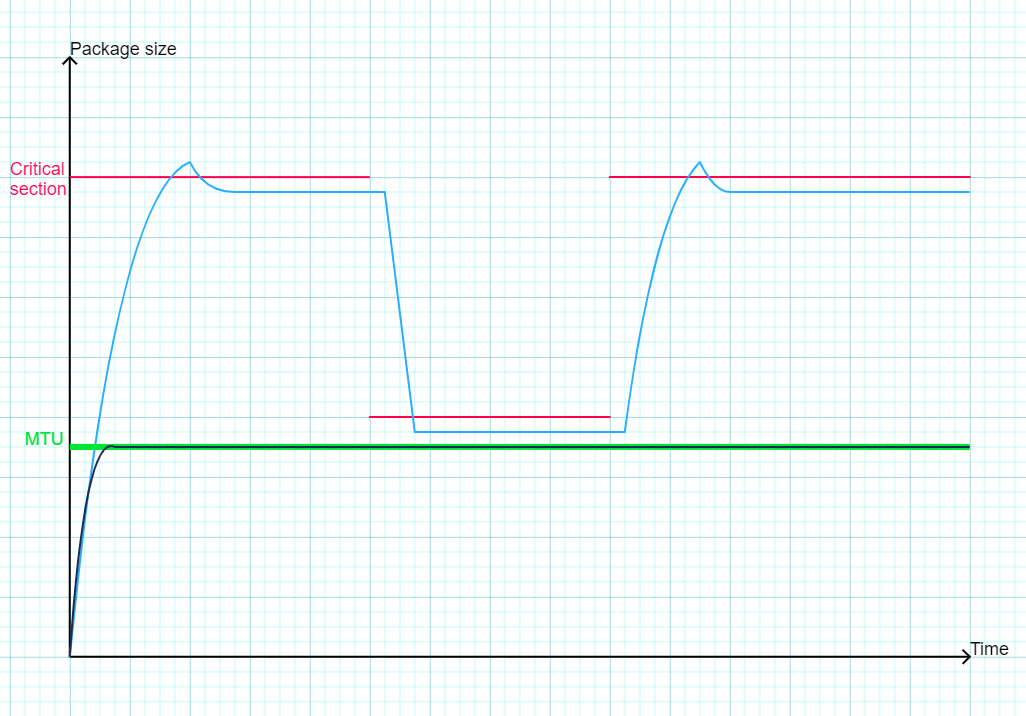
\includegraphics[scale=0.5]{9/09_01.png}
	\caption{Оптимизация TCP по размеру пакетов}
	\label{fig:graph_9}
\end{figure}

На рисунке~\ref{fig:graph_9} наглядно проиллюстрирован данный процесс. Красной линией отмечена \textit{критическая секция}, а голубой - график изменения размера пакетов данных по мере их передачи.

Пример работы при заданном параметре MTU (зелёная линия) отображён тёмно-синей кривой.

\textcolor{red}{\textbf{Внимание!}} Данный график является лишь схематической иллюстрацией и не претендует на точность.

\bigskip 
Представим бытовую ситуацию: у нас дома есть WI-Fi роутер, подключённый к сети Интернет, и к этому роутеру в квартире подключены ПК, ноутбук, планшет, телефоны и ещё несколько устройств. С точки зрения внешней сети (Интернет) существует лишь роутер со своим IP-адресом. С точки зрения роутера, есть внешняя сеть + все устройства, которые находятся дома (у каждого из них есть свой локальный адрес, уникальный в этой локальной (домашней) сети). Тогда как нам отделять входящие и исходящие запросы, предназначаемые для ноутбука, ПК и прочих устройств по отдельности?

В решении этой задачи и заключается суть технологии \href{https://ru.wikipedia.org/wiki/NAT}{NAT}. Принимая пакет от локального компьютера, роутер смотрит на IP-адрес назначения. Если это локальный адрес, то пакет пересылается другому локальному компьютеру. Если нет, то пакет надо переслать наружу в интернет. Но ведь обратным адресом в пакете указан локальный адрес компьютера, который из интернета будет недоступен. Поэтому роутер «на лету» транслирует (подменяет) обратный IP-адрес пакета на свой внешний (видимый из интернета) IP-адрес и меняет номер порта (чтобы различать ответные пакеты, адресованные разным локальным компьютерам). Комбинацию, нужную для обратной подстановки, роутер сохраняет у себя во временной таблице. Через некоторое время после того, как клиент и сервер закончат обмениваться пакетами, роутер сотрёт у себя в таблице запись об n-м порте за сроком давности.

NAT меняет лишь заголовок и не трогает само ''тело'' передачи (посылает пакеты в таком виде, в каком их получил). Из-за этого сама по себе пересылка данных является незащищённой (то есть, если вы захотите переслать пароли с одного сервера на другой через Интернет, то потенциальный злоумышленник сможет их прочитать где-то по пути передачи).

\bigskip    
Для построения защищённых каналов связи используется \href{https://ru.wikipedia.org/wiki/VPN}{VPN}. Представим, что у нас есть два сервера, у каждого из которых какой-то свой закрытый контур (внутри которого уже используется, например, NAT), и мы хотим провести между ними соединение через Интернет. VPN помогает установить сетевое соединение поверх сети Интернет, создавая защищённый канал, проходя через который, данные будут шифроваться на входе и расшифровываться на выходе.
Таким образом, даже если потенциальный злоумышленник захочет прочитать эти данные (да, он всё ещё может где-то по пути пересылки данных увидеть их), то не сможет, ведь они зашифрованы. Недостатком VPN, очевидно, является скорость, ведь шифровать и расшифровывать данные - не самая быстрая операция.
\newpage
\section {Билет 10. Методы обеспечения отказоустойчивости. RAID, распределенное хранение данных, виды и репликаций.}
\newpage
\section {Билет 11. Методы шифрования данных.}
В курсе было рассмотрено два метода шифрования 
\begin {itemize}
\item симметричное (т.е. для шифровки и дешифровки используется один и тот же ключ) или с закрытым ключом 
\item асимметричное (т.е. для шифровки и дешифровки используются разные ключи) или с открытым ключом
\end {itemize}

Далее будет использоваться следующая терминология: мы хотим отправить по открытому каналу связи сообщение $X$, нам его нужно зашифровать, чтобы злоумышленник, просматривающий канал связи, не смог прочитать передаваемое сообщение. Зашифрованное сообщение будем обозначать через $Y$. Степень невозможности прочтения исходного текста, полученного из канала связи в виде шифра, зависит, как правило, от некоторой небольшой информации, имеющейся у отправителя и получателя ее (быть может, различной) и называющейся ключом $K$.

\subsubsection{Симметричное}
\href{https://clck.ru/9KE6e}{Шифр Цезаря} \\
Пусть отправляемое сообщение $X$ составлено из алфавита $A$. Простым шифром подстановки называется шифр вида:

$$ X = (x_1, x_2, \dots x_n), Y = (\sigma (x_1), \sigma(x_2), \dots \sigma(x_n)), \, \text{где}\, \sigma - \text {перестановска букв алфавита А} $$

В оригинальном шифре Цезаря использовался циклический сдвиг на 3 позиции левее. Приведем простой пример: пусть сообщение $X$ имеет вид "Съешь же ещё этих мягких французских булок, да выпей чаю", тогда сообщение $Y$ будет выглядеть "Фэзыя йз зьи ахлш пвёнлш чугрщцкфнлш дцосн, жг еютзм ъгб" \\

Все шифры простой замены не устойчивы к взлому (и шифр Цезаря не исключение). В каждом языке одни буквы встречаются часто, а другие - редко. Например, в русском языке самая часто употребляемая буква о, а самая редко употребляемая ф. И эта тенденция сохраняется практически в любом тексте русского языка. Поэтому, можно провести частотный анализ зашифрованного текста $Y$, т.е. посчитать частоту вхождения каждой буквы и соотнести частоты букв зашифрованного текста с общеизвестными частотами букв русского языка.\\
\\
\href{https://clck.ru/TQFhp}{Шифр Вернама} \\
Пусть сообщение $X$ - вектор длины n состоящий из 0 и 1 ($X \in \{0, 1\}^n$), ключ $K$ - выберем такой же длины n, $K \in \{0, 1\}^n$. Тогда зашифруем сообщение $X$ следующим образом: $X \oplus K = Y$, где $\oplus$ - сложение по модулю два происходит покомпонентно. Этот вид шифрования прост и очень надежен, но если к злоумышленнику попадет сообщение $X$ и $Y$, то можно просто найти ключ $K$ так как $K = X \oplus Y$. Поэтому на практике используют другой подход: пусть хотим передать сообщения $X_1, X_2, X_3 \dots X_n$, пусть выбран какой-то ключ $K_1$, и шифр $Y_1$ получается по правилу $Y_1 = X \oplus K$. Тогда на шаге $i$ ключ $K_i = f (K_{i - 1}, X_i, \dots X_1)$, где $f()$ - некоторая функция. Тогда даже, если будет перехвачен $Y_i$ и $X_i$ и будет получен $K_i$, то предыдущие сообщения останутся не расшифрованными, так как они кодировались другими ключами. \\
\\
\href{https://clck.ru/UNdXg}{Блочный шифр} \\
Пусть есть последовательность сообщений одинаковой длинны $X_1, X_2, X_3, \dots X_n, X_i \in \{0, 1\}^n$ которую мы хотим передать по открытому каналу связи. Пусть есть последовательность пар $(\sigma_1, K_1), (\sigma_2, K_2), \dots (\sigma_i, K_i) \dots$ где $\sigma$- это перестановка на множестве букв алфавита $A$, $K_i$ - вектор из 0 и 1, $K_i \in \{0, 1\}^n$. Тогда ключом мы назовем последовательность пар т.е. $K = ((\sigma_{i_1}, K_{i_1}), (\sigma_{i_2}, K_{i_2}), (\sigma_{i_n}, K_{i_n}))$ и шифрование происходит так: сначала к сообщению $X_1$ применяется перестановка букв $\sigma_{i_1}$, к результату применяется шифр Вернама с ключом $K_{i_1}$ и так далее, к сообщению $X_2$ применяется перестановка $\sigma_{i_2}$, потом шифр Вернама с ключом $K_{i_2}$ и т.д.

Возникает логичный вопрос, как передать ключ для расшифровки? \\

\subsubsection{Способы передачи ключа}

\begin {itemize}
\item Пусть по открытому каналу связи общаются Алиса (A) и Боб (B) им нужно передать ключ. Пусть есть две функции $f_{A}, f_{B}$ к которым известны обратные $f^{-1}_{A}, f^{-1}_{B}$ и которые обладают свойством $f_{A} (f_{B} (x)) = f_{B} (f_{A} (x))$. Тогда для передачи ключа $k$ от A к B используется следующий алгоритм:
\begin {itemize}
\item A отправляет B сообщение $f_{A} (k)$ 
\item B отправляет A сообщение $f_{B}(f_{A} (k))$
\item A отправляет B сообщение $f^{-1}_{A}(f_{B}(f_{A} (k)))$
\item B применяет к сообщению $f^{-1}_{B}$ и получает $f^{-1}_{B}(f^{-1}_{A}(f_{B}(f_{A} (k)))) = k$
\end {itemize}
В качестве $f_{A}, f_{B}$ - используют функции возведения в степень по модулю \\

\item \href{https://clck.ru/9rNPo} {Протокол Диффи—Хеллмана}\\
Не всегда требуется передать ключ от одного пользователя к другому, иногда достаточно выработать единый. 
\begin {itemize}
\item А придумывает $N$ - модуль по которому будут проводится сравнения, $a, X$ - вычеты по модулю $N$. A отправляет В пару $(X, N, X^{a} \, (mod \, N))$
\item B придумывает показатель $b$ и отправляет А $X^{b}$
\item В итоге у А и В формируется одинаковое число $\left( X^{b} \right)^{a}$
\end {itemize}
\end{itemize}
На первый взгляд можно подумать, что взлом схемы очевиден, ведь достаточно знать показатели степени $a, b$, а для этого необходимо лишь прологарифмировать сообщения $X^a, X^b$ так как мы знаем сообщение $X$ - то можно узнать и показатель. Но не существует эффективного поиска логарифма числа по модулю $N$ (см. \href{https://clck.ru/pv4S6}{Дискретный логарифм}). Поэтому на практике данная процедура займет бесконечно много времени.

\subsubsection{Асиметрические алгоритмы (Алгоритмы с открытым ключом)}

В лекциях был разобран  RSA алгоритм. Задача формулируется аналогичным образом: мы хотим отправить по открытому каналу связи сообщение $X$, нам его нужно зашифровать, чтобы злоумышленник, просматривающий канал связи, не смог прочитать передаваемое сообщение. \\

Перед тем как рассказать суть RSA алгоритма вспомним теорему Эйлера. \\
Теорема (Эйлер). Если Числа X и N взаимнопросты, то тогда $X^{\varphi (N)} \, = \, 1 \, (mod \, N)$ \\
$\varphi$ - функция Эйлера. Например, для простого числа $p$ его функция Эйлера $\varphi (p) = p - 1$ \\

Вспомним давних товарищей, общающихся по каналу связи, Алису (A) и Боба (B). Пусть сообщение передает Боб.
Алиса берет число $N = pq$, p,q - различные простые числа. Тогда $\varphi (N) \, = \, (p - 1)(q - 1)$. И подбирает число $e$ так, чтобы $(e, \varphi(N)) \, = \,1$. С помощью Алгоритма Евклида ищется $d$ такое, что  $ed = 1 (mod \, \varphi (N))$. Тогда сам алгоритм выглядит следующим образом:
\begin {itemize}
\item A передает В пару $(N, e)$. e - открытый ключ, d - секретный.
\item B передает сообщение $X^e$
\item A полученное сообщение возводит в степень $d$ т.е. $(X^e)^d = X (mod N)$
\end {itemize}

Злоумышленник не может перехватить сообщение $X$ по двум причинам: сложность разложения числа $N$ на простые множители (так как надо по числу $e$ определить число $d$, для этого нужно посчитать функцию Эйлера, а для этого нужно разложить число на простые множители, чтобы воспользоваться свойствами мультипликативности функции Эйлера) и проблема дискретного логарифма.

\subsubsection{Цифровая подпись}

Как Алисе убедить Боба, что она автор сообщения $X$? Очень просто. Пусть как в предыдущем пункте Алиса выберет $e, d, N$ так, чтобы $ed \, = \,1 \,(mod \, \varphi (N))$. Тогда в открытом доступе Алиса публикует пару $(e, N)$ и  $(X, X^d)$. Боб делает проверку: берет $X^d$ из открытого доступа и возводит в степень $e$ и смотрит совпадает ли полученное сообщение с $X$  т.е. выполнено ли, что $X \, = \, (X^d)^e \, (mod \, \varphi (N))$. На этом простом примере основан принцип электронной (цифровой) подписи. Электронная подпись - позволяет подтвердить авторство электронного документа. Например, Алиса при отправке сообщения $X$ Бобу, сначала отправляет сообщение в "Удостоверяющий Центр", который генерирует числа $e, d, N$. "Центр" пересылает Бобу пару $(X, X^e)$, а Боб с помощью открытого ключа проверяет, что документ отправлен Алисой. Удостоверяющие центры могут выстраиваться по иерархии, и центры находящиеся выше, подтверждают подписи накладываемые центрами ниже.






\newpage
\section {Билет 12. Полнотекстовый поиск. Алгоритмы без индексов. Поиск с реверсивным индексом.}
\begin{defn}
Текстом назовем произвольный упорядоченный набор слов в некотором алфавите. Фрагмент текста или просто фрагмент — поднабор текста, в который входят подряд идущие слова с сохранением порядка. \end{defn}
\href{https://clck.ru/pwwdR}{Полнотекстовый поиск} - автоматизированный поиск документов, при котором поиск ведётся не по именам документов, а по их содержимому, всему или существенной части.

\subsection{Безиндексный поиск}
В этом пункте мы рассмотрим поиск с помощью регулярных выражений. Подробнее можно прочитать тут:\href{https://habr.com/ru/company/vk/blog/270507/}{regex}. Регулярные выражения - так называют способ описания шаблонов строковых данных. Если некий набор строковых данных аналогичен тому, что описывается регулярным выражением (РВ), то мы говорим о совпадении РВ с этими строковыми данными.

Простейшим случаем регулярного выражения является одиночный буквенный символ. За исключением метасимволов — $*, +, ?, (, ),|,$ — все символы равны сами себе. Для поиска совпадений с метасимволами нужно добавлять обратный слеш: комбинация символов $\backslash +$ аналогична +.

Два регулярных выражения могут преобразовываться или объединяться, создавая новое регулярное выражение: если E1 соответствует S, а E2 соответствует t, тогда E1|E2 соответствует S или T, а E1E2 соответствует ST.

Метасимволы *, + и? являются операторами цикла:
\begin {itemize}
\item E1* говорит о том, что E1 может встречаться 0 и более раз;
\item E1+ говорит о том, что E1 может встречаться 1 и более раз;
\item E1? говорит о том, что E1 может встречаться 0 или 1 раз.
\end {itemize}

Грубо говоря, регулярный язык представляет собой набор строк, которые могут быть найдены в тексте за один проход с использованием фиксированного объёма памяти. Современные реализации регулярных выражений (в Perl и ряде других языков) используют многочисленные новые операторы и управляющие последовательности. Реализация поиска строки использует понятие конечного автомата, они также известны как машины состояний (state machines). 

\subsection {Реверсивный индекс}
Пусть у нас выборка текстов $T_1, T_2 \dots T_{N}$, занумерованных натуральными числами. Есть несколько ключевых слов $k_1, k_2, \dots k_n$ и есть файлы $F_1, \dots F_n$. В файле $F_i$ записаны номера текстов, в которых встречается слово $k_i$. Приведем пример, пусть есть два слова СТОЛ, СТУЛ, и файлы $F_1, F_2$  имеют вид: \\
$$ F_1: 1,3,4,7,9 $$
$$ F_2: 2,3,4,5,6,8 $$

Пусть номера текстов в файлах отсортированы!
Тогда алгоритм поиска прост: мы производим сливание отсортированных массивов (соответственно, если нам нужно найти слова СТОЛ И СТУЛ, то выбираем файлы в которые входят оба эти слова, если  СТОЛ ИЛИ СТУЛ, то просто сливаем два массива). Так как массивы в файлах отсортированы, то задача слияния выполняется быстро.\\
Вопрос: если один файл изменили, что делать ? Например, в 1 тексте слово ТАБУРЕТКА заменили на СТУЛ. Текст 1 попадает в специальный файл, где хранятся удаленные тексты, а номер 1 заменяется, например, на 10 (Подбор номера происходит не произвольным образом, а заменяется на максимальный неиспользованный номер). Тогда:
$$ F_1: 3,4,7,9, 10 $$
$$ F_2: 2,3,4,5,6,8,10 $$
$$DEL (\text{удаленные}): 1$$

Если в 4 файле заменили, слово СТУЛ на ТАБУРЕТКА, то (номер 4 заменяем на 11) имеем:
$$ F_1: 3,7,9, 10, 11 $$
$$ F_2: 2,3,5,6,8,10 $$
$$DEL (\text{удаленные}): 1, 4$$

Когда все номера становятся очень большими, их все можно уменьшить.
\newpage
\section {Билет 13. Обработка текстов. Морфологический анализ, tf*idf, ранжирование, исправление опечаток, классификация, кластеризация, поиск дубликатов.}

Пусть у нас есть пачка текстов $T_1, T_2, T_3 \dots T_n$, которую мы будем исследовать \\
Методы представления текстов
\begin{itemize}
\item множественный. Текст представляется как множество слов, для которых не определено отношение порядка. Преимущество - простота. Для вычисления сходства двух текстов используется простая формула $k = \frac {|A \cup B|}{|A \cap B|}$. Если коэффициент большой, то тексты похожи друг на друга.
\item векторная модель. Пусть есть выделенные  "базисные" слова $w_1, w_2, \dots w_n$, тогда текст представляется вектором в n-мерном пространстве, где, в простейшем случае, координаты вектора строятся так: i - ая координата это количество вхождения слова $w_i$ в текст. Но на практике используют другой способ определения координат (способ с помощью модели tf*idf)  
\end{itemize}

\subsubsection {Модель tf*idf для построения векторов}
\href{https://clck.ru/EqWAS}{Векторная модель} \\
\underline {Определение}
tf для слова $w_i$ в тексте $T_j$ определяется так: 
 $tf = log (Q)$, Q - сколько раз $w_i$ встретилось в $T_j$.  \\
idf для слова $w_i$ в тексте $T_j$ определяется так: 
$idf = \frac{1}{log(P)}$, P - количество документов в последовательности $T_1, T_2, T_3 \dots T_n$, в которых встречается слово $w_i$ \\
На практике используют именно произведение $tf*idf$ - означающее важность слова в документе. Произведение tf*idf отражает закон Зипфа:
На графике по вертикальной оси откладывается важность (т.е. tf*idf) по горизонтальной частота встречаемости слова в конкретном документе. 
Выделяется три зоны: \\
1 - редкие слова, слова придуманные автором или опечатки \\
2 - ключевые слова, определяющие текст \\
3 - обычные слова связки \\

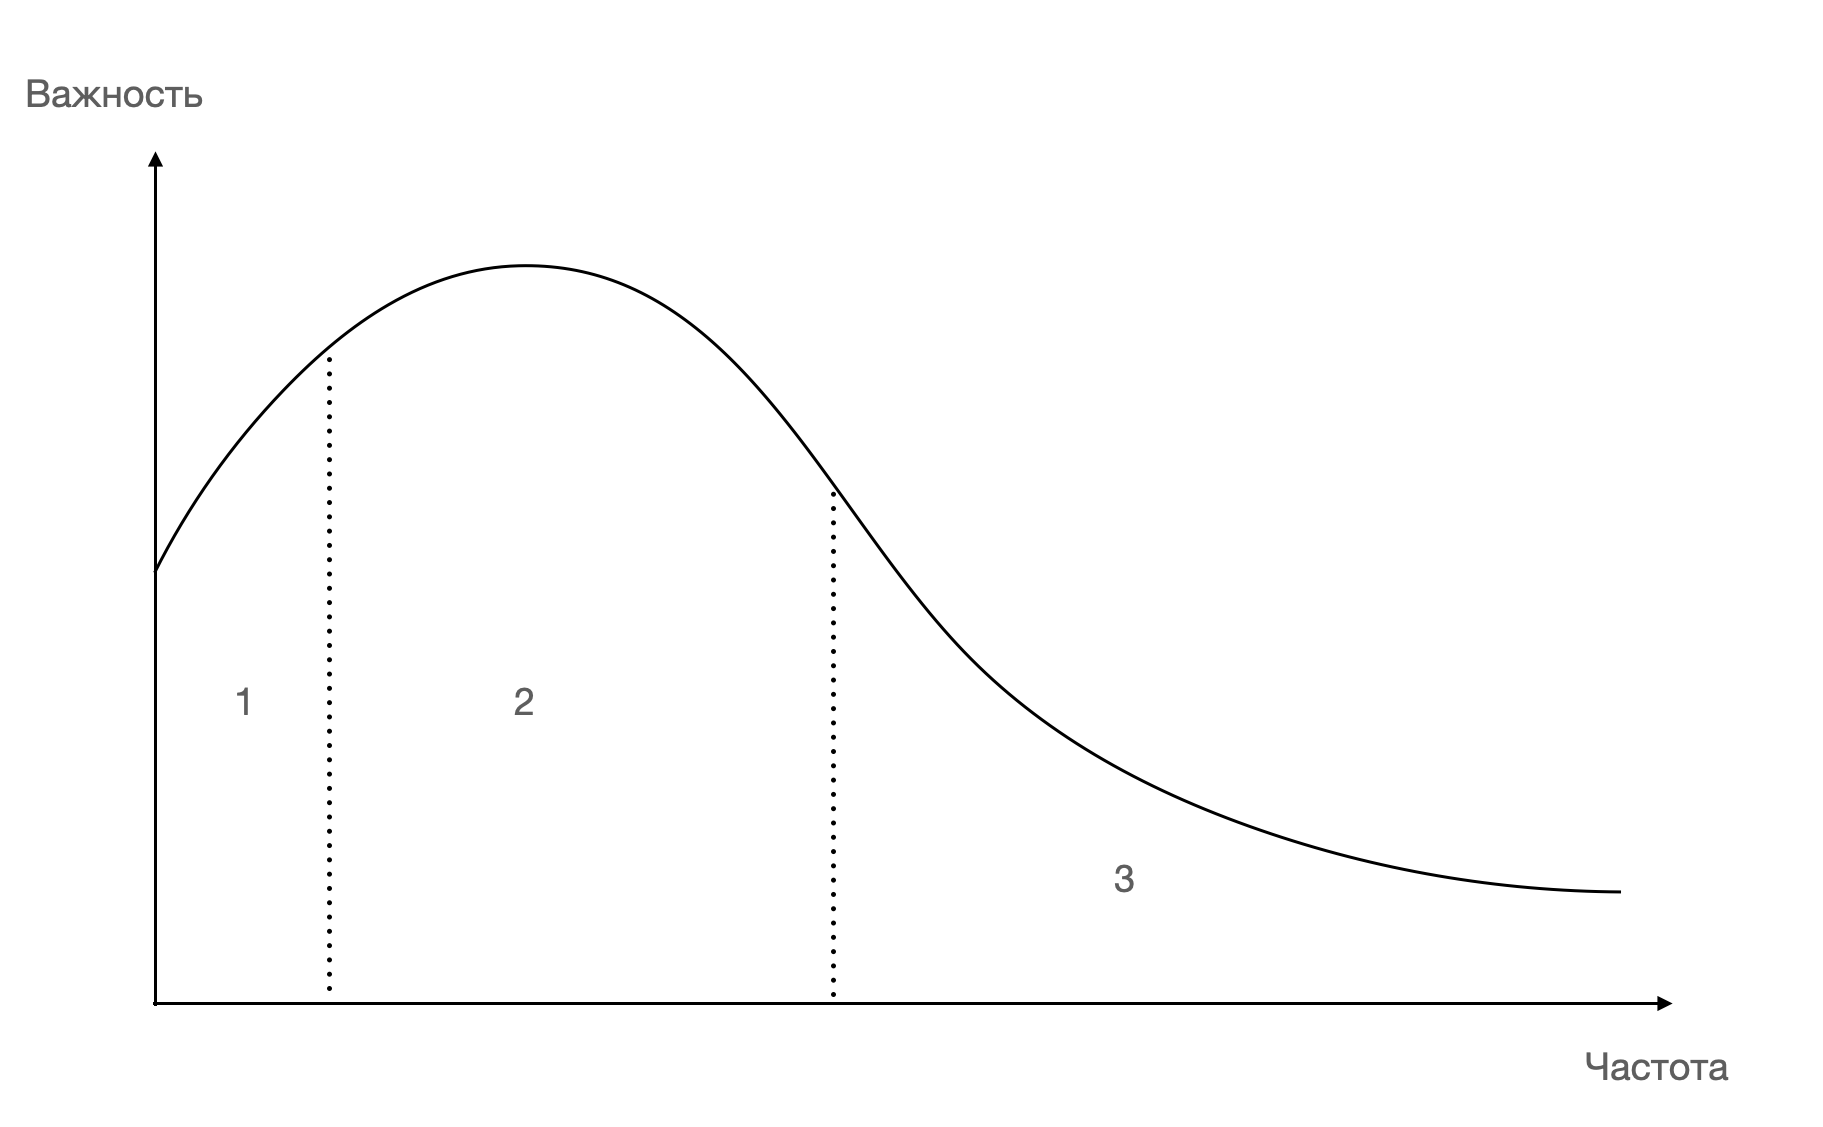
\includegraphics[width=0.5\linewidth]{13/Zipf}
Поэтому, в итоге, текст это вектор, где на i - ом месте стоит tf*idf слова $w_i$. Мера близости текстов A и B в векторной модели - косинус угла между векторами A и B.

\subsubsection {Морфологический анализ}
\href{http://prutzkow.com/ru-ru/science/natural-language-processing/morphology/}{Морфологический анализ} \\
Перед построением векторов сначала несколько унифицируют используемые слова, для этого используют морфологический анализ.
Морфологический анализ может быть словарным (со словарем основ и окончаний или словарем словоформ) или бессловарным (только со словарем окончаний; словарь окончаний может быть встроен в алгоритм морфологического анализа). Бессловарный метод используется только для определения переменной морфологической информации (не всегда однозначно), а словарный — во всех остальных случаях. 

\subsubsection {Исправление опечаток}
\href{https://clck.ru/A6RjQ}{Расстояние по Левенштейну} \\
Элементарная операция по Левенштейну - это добавление буквы, удаление буквы или замена одной буквы на другую. Расстояние это количество операций необходимое для того, чтобы из одного слова получить другое с помощью операций Левенштейна. Например, слова aabb, aabbb, aab, aacb находятся на одинаковом расстоянии (расстояние равно 1). Далее, чтобы исправить опечатку необходимо найти ближайшее слово по Левенштейну. Если использовать обычный, линейный поиск то процедура поиска может занять много времени. Поэтому используют поиск по дереву. В вершинах дерева расположены буквы, различные пути образуют слова. 

\subsubsection {Поиск дубликатов}
Если необходимо решить задачу на полное совпадение текстов, то она делается очень просто. Для каждого документа берется хэш-функция (например, MD5). С большой вероятностью документы с совпадающем значение хэш-функции - совпадают. Но на практике необходимо искать не в точности совпадающие тексты, а просто похожие. В таком случае используют понятие N-грамм.  \\
\underline {Определение:} N-грамма — последовательность из N элементов. Например для текста: Мама мыла раму, все 4 граммы имеют вид: мама, амам, мамы, амыл, мыла, ылар, лара, арам, раму.  \\
\underline {Теорема.} Если документы почти совпадают, то и N-граммы почти совпадают\\
Это отличный способ - сравнивать все N-граммы, но есть одна проблема - их очень много и сравнение всех N-грамм двух текстов займет много времени. Поэтому действуют следующим образом.

\begin {itemize}
\item Берутся все N-граммы двух текстов и к ним применяется какая-нибудь хеш-функция (Например, \href{https://clck.ru/9cRa4}{MD5}). (хэш-функция от N - граммы называется называется шинглом)
\item Береться 84 шингла (значения хэш-функции), они объединяются в 12 групп.
\item На каждой группе шинглов опять вычисляется хэш-функция. (значение хэш функции на группе шинглов называется супершинглом)
\item Если у двух текстов совпадает хотя бы один супершингл,  то они потенциально совпадают.
\end {itemize}

\subsubsection {Классификация и кластеризация}
Классификация - разделение текстов на группы, которые мы заранее определили. Кластеризация - разделение на группы, заранее не известные.
Примеры разделения: по авторству, по эмоциональной окраске текста, по цели (повествование/реклама), по различным темам.
Описанные ниже методы одинаково применяются для кластеризации и классификации.

\begin {itemize}
\item Тезаурус. Берется двудольный граф, в котором в одной доле (будем ее называть доля  W) располагаются термины, а во второй доле - темы (будем ее называть T). Вершина из W соединяется с вершиной из T, когда соответствующий термин описывает данную тему, на ребре соединяющем вершины приписывается число меньшее 1, показывающее степень соответствия термина теме (Например, термин "матрица" однозначно соответствует линейной алгебре, но может встречаться и в теории вероятностей (но встречается там гораздо реже, чем в линейной алгебре), тогда на ребре матрица-линейная алгебра будет, например, 0.7, а на ребре матрица-теория вероятностей -- 0.3 ). То есть в итоге имеем взвешенный двудольный граф. Данный граф дается нам лингвистами или формируется нами. Далее мы читаем полученный текст и если встречаем термин w из W, который соединен ребром веса p с темой t, то к теме t  прибавляем соответствующий вес p. Тема у которой в результате чтения текста будет максимальное значение - тема текста. Минус этого метода: необходимо строить хороший двудольный граф, т.е. отвечающий современному состоянию языка.
\item Самообучающиеся карты.
Пусть стоит задача разделить цветные точки на группы так, чтобы в каждой группе были точки одного цвета. В начальный момент времени все точки расположены в трехмерном пространстве хаотично (Почему трехмерном? Каждый цвет однозначно представляется тремя числами в системе rgb (rgb - аддитивная цветовая модель, описывающая способ кодирования цвета для цветовоспроизведения с помощью трёх цветов, которые принято называть основными)). Выбираются функции $f_1, f_2, f_3$ как показано на рисунке (Функции определены на отрезке $[-3, 3]$ и интегралы $\int_{-3}^3 f_i (x) dx$ = 1 (На уровне идеи это требование означает, что цвет суммарно не меняется)).
Далее используется следующий алгоритм:
\begin {itemize}
\item Для точки A в ее окрестности считается сумма $S = \sum_{p_i \in U} c (p_i) f_1 (\rho_i)$, где $U$ - окрестность точки A, $p_i$ - точки, принадлежащие этой окрестности, $c (p_i)$ - цвет точки $p_i$ (вектор в трехмерном пространстве), $\rho_i$ - расстояние от точки $p_i$ до точки A. Точка А красится в цвет S. Так последовательно делаем для всех точек. Может получится так, что цвета $S$ - не было среди цветов изначальных точек, но это нормально.
\item Проделываем процедуру еще раз с функциями $f_2, f_3$
\item В итоге все точки разделяться на группы, причем например, между синим и зеленым цветом будет желтый, а между синим и красным - фиолетовый.
\end {itemize}

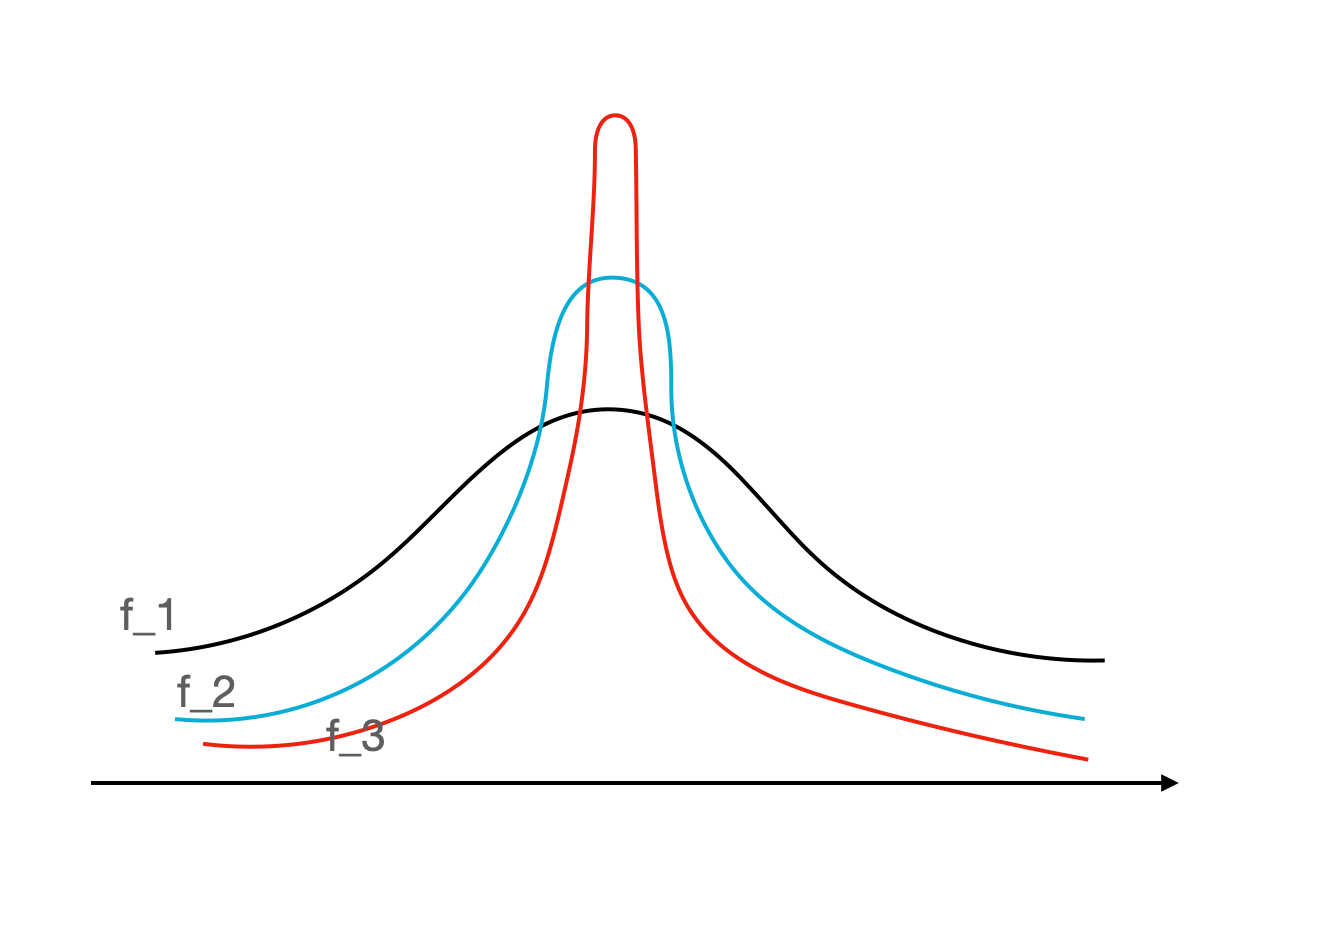
\includegraphics[width=0.5\linewidth]{13/func}

\begin{figure}[h!]
\begin{minipage}[h]{0.49\linewidth}
\center{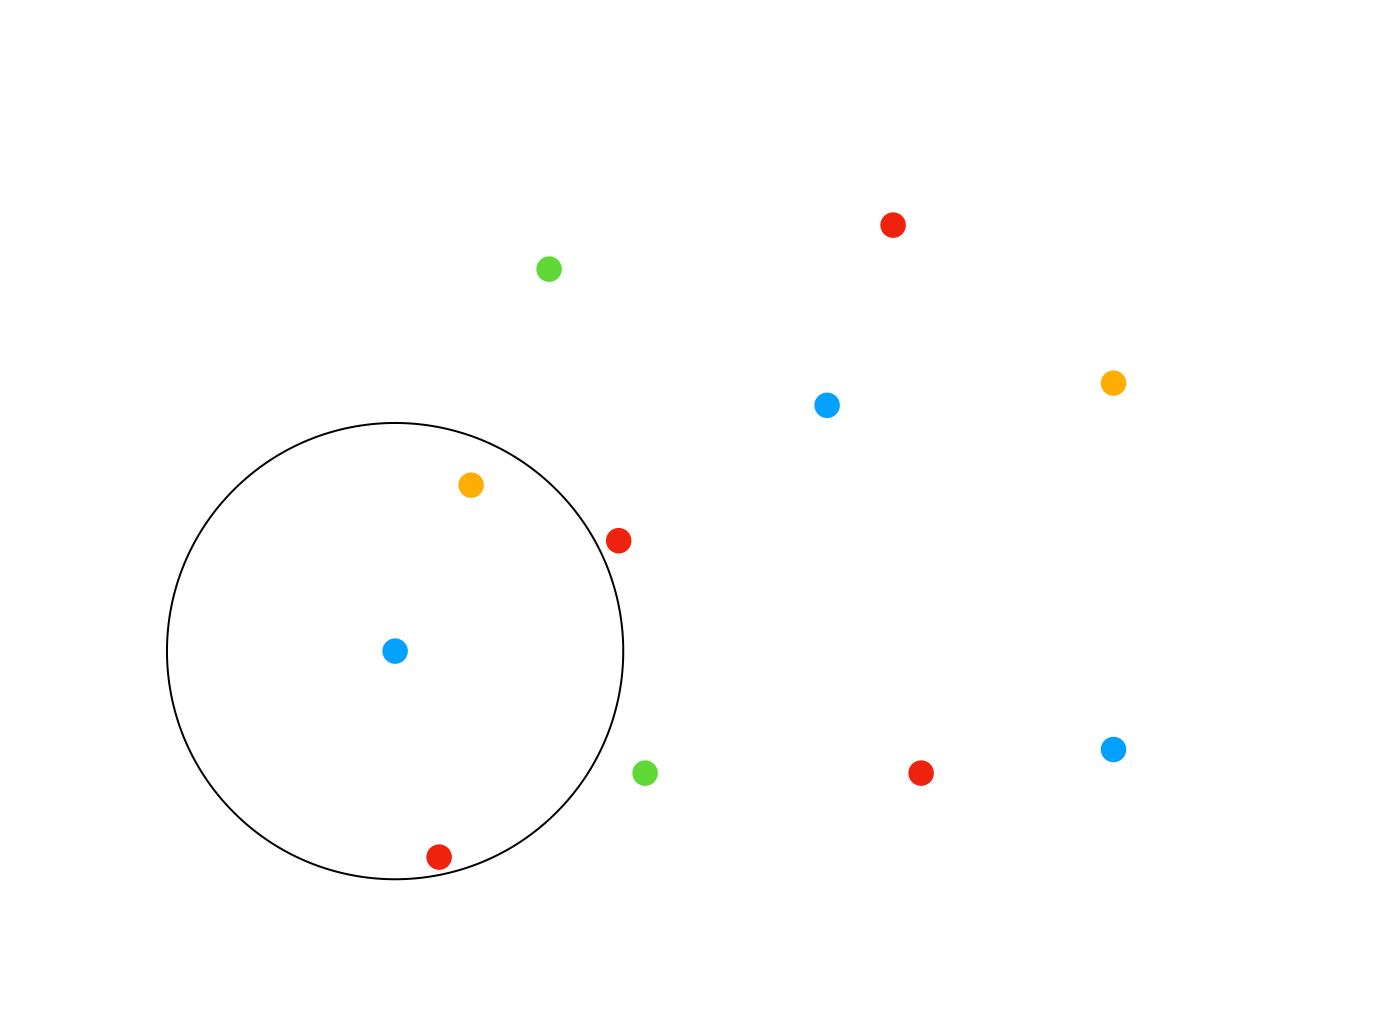
\includegraphics[width=\linewidth]{13/begin} положение точек до работы алгоритма \\}
\end{minipage}
\hfill
\begin{minipage}[h]{0.49\linewidth}
\center{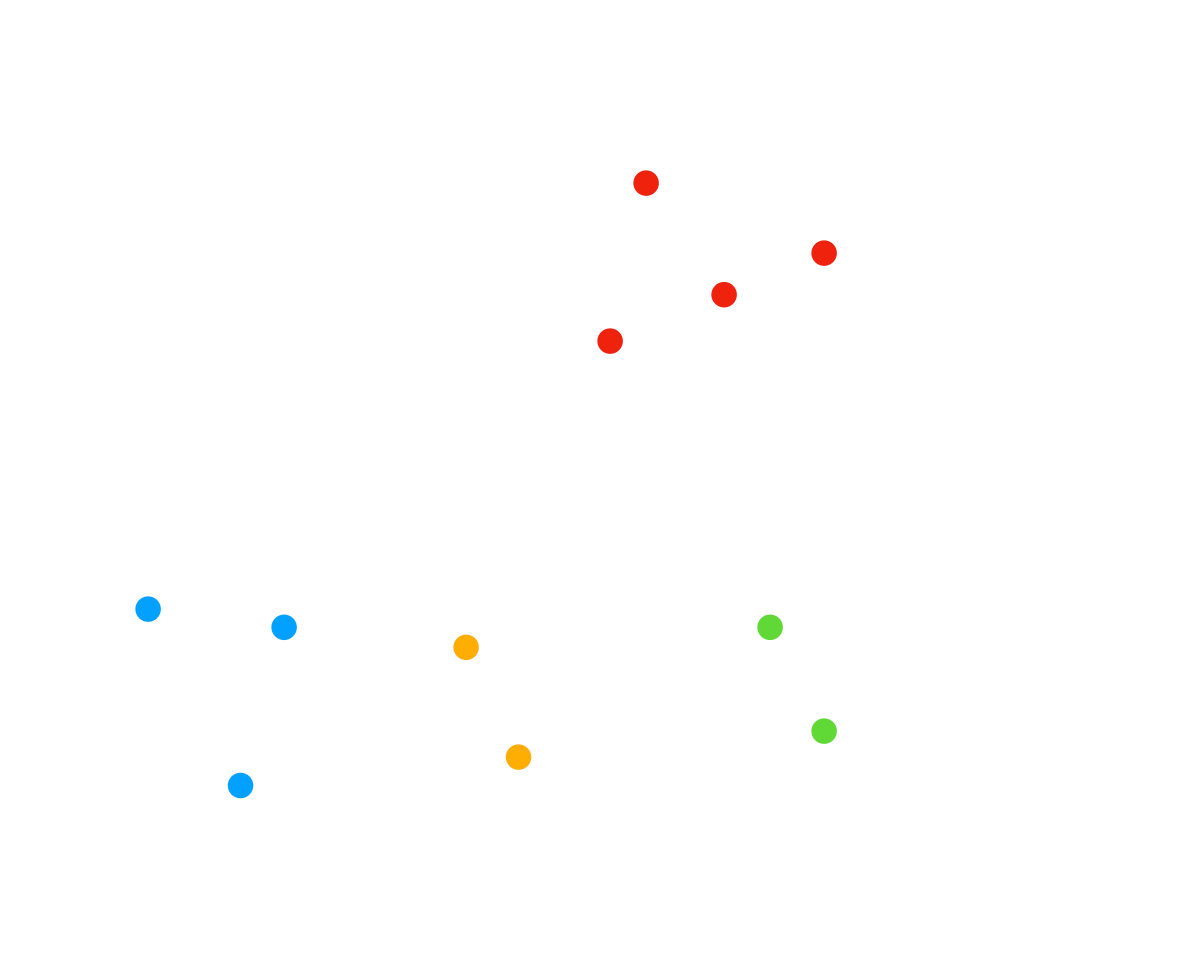
\includegraphics[width=\linewidth]{13/result} положение точек после работы алгоритма \\}
\end{minipage}
\end{figure}

\item  Физическая расстановка.
Стоит задача разделит точки на группы. Припишем каждой точке свою массу. Зададим векторы силы всемирного тяготения по формуле 
$\vec{F_{A,B}} = G \frac{m_{A} m_{B}\vec{r}}{|\vec{r}|^3}$, где $G$ - константа, $\vec{r}$ - вектор соединяющий точки А и В, $m_{A} m_{B}$ - массы точек. Тогда за время $\Delta t$ каждая точка под действием равнодействующей силы притяжения передвинется на расстояние $\Delta s_i$ (свое для каждой точки). Если точки находятся близко, то объединяем их в одну точку суммарной массы. Алгоритм проводится до тех пор пока нас не удовлетворит разделение на группы или точки не попадут в равновесное состояние.  

\item Геометрическая расстановка. (Наиболее часто встречаемый метод). Пусть есть точки на плоскости которые мы хотим объединить в группы. (см. рисунки шаг 1-4)
\begin{itemize}
\item на шаге 1 имеем просто хаотично разбросанные точки.
\item на шаге 2 в произвольные места добавляем точки-кластеры, которые отвечают за образование групп.
\item на шаге 3 определяем какие точки к какому кластеру ближе.
\item на шаге 4 перемещаем кластеры в центр масс соответствующих точек и применяем шаг 3 к новой конфигурации.
\item шаг 4 продолжаем до тех пор пока кластеры не перестанут двигаться.
\end{itemize}

\begin{figure}[h]
\begin{minipage}[h]{0.47\linewidth}
\center{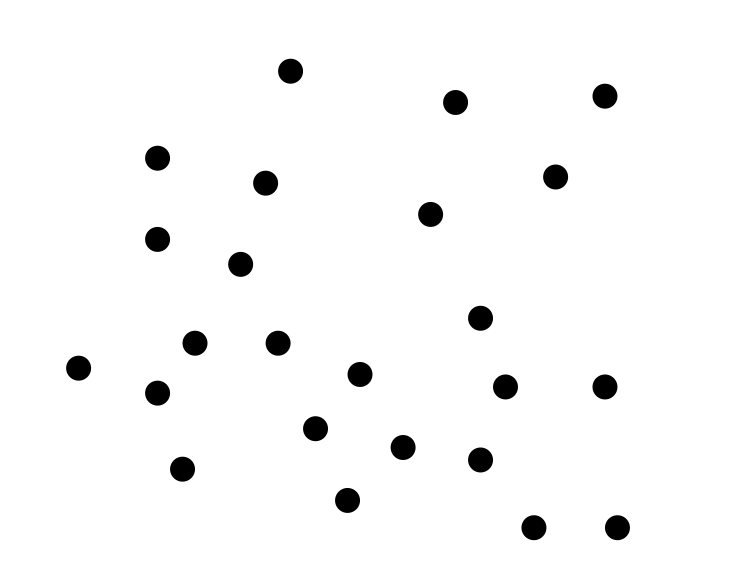
\includegraphics[width=1\linewidth]{13/1}}  \\ шаг 1
\end{minipage}
\hfill
\begin{minipage}[h]{0.47\linewidth}
\center{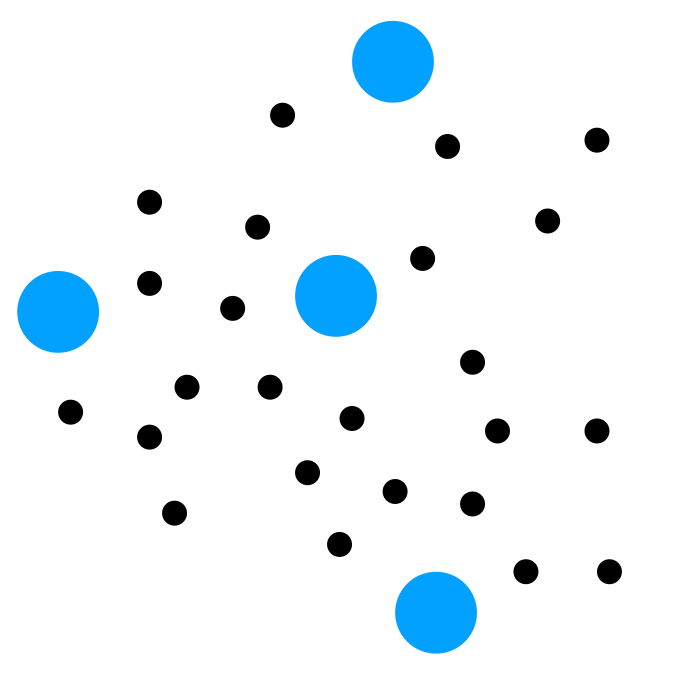
\includegraphics[width=1\linewidth]{13/2}} \\ шаг 2
\end{minipage}
\vfill
\begin{minipage}[h]{0.47\linewidth}
\center{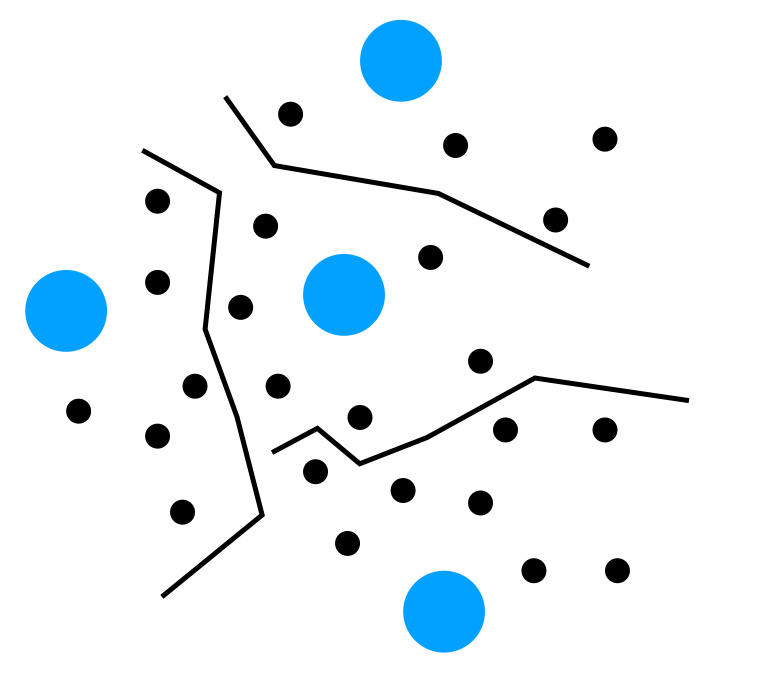
\includegraphics[width=1\linewidth]{13/3}} \\ шаг 3
\end{minipage}
\hfill
\begin{minipage}[h]{0.47\linewidth}
\center{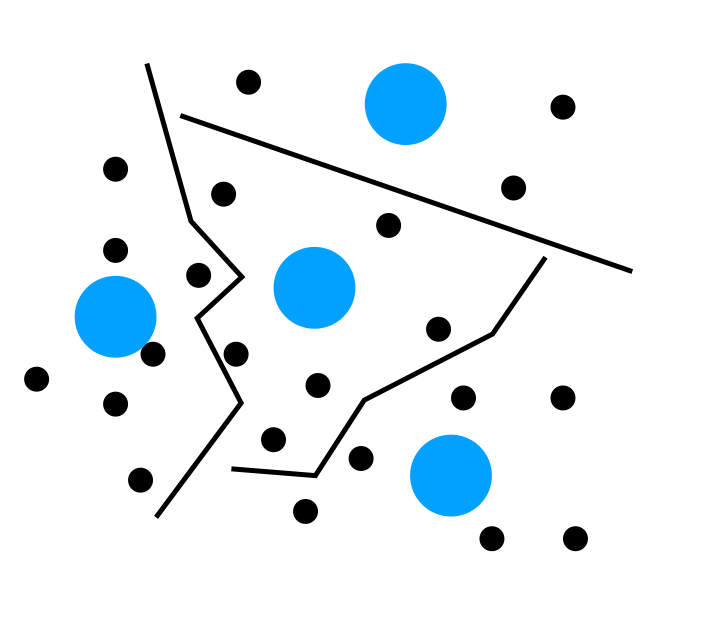
\includegraphics[width=1\linewidth]{13/4}} \\ шаг 4
\end{minipage}
\end{figure} 

После работы алгоритма, точки находящиеся вблизи соответствующего кластера, объединяем в группы.
\end{itemize}

\subsubsection {Ранжирование}
Зачастую на запрос пользователя подходит несколько документов, набор подходящих документов будем называть коллекцией. Как выбрать один, наиболее подходящий? Для этого считают функцию ранжирования: $R = S A$.
\begin{itemize}
\item $S$ - функция соответствия запросу. Как обсуждалось выше это может быть косинус угла между текстом и запросом или например \href{https://clck.ru/pvLYk}{BM25}, которая определяется следующим образом: Пусть запрос $Q$ состоит из слов $q_1, q_2, \dots q_n$ тогда $$ s = \sum_{i = 1}^n idf (q_i)
 \frac {f(q_i, D)(k_1 + 1)}{f(q_i, D) + k_1 \times \left(1 - b + b \frac{|D|}{avgdl} \right)} $$ где $n$ - количество слов в запросе, $idf(q_i)$ - idf слова $q_i$, $f(q_i, T)$ - частота слова $q_i$ в тексте $D$, $|D|$ - количество слов (мощность) текста $D$, avgdl - средняя длина слова в коллекции документов, $k_1 = 2.0, b = 0.75$. 
\item A - функция авторитетности конкретного документа (эта функция своя для каждого документа и ее значение не зависит от запроса). Приведем пример определения авторитетности: Пусть есть ссылочный граф, т.е. в вершинах графа тексты и если текст A ссылается на текст B, то в графе есть соответствующее ребро. Запустим в граф робота, который будет ходить по графу по следующему правилу: с вероятность p робот переходит из вершины в которой находится в одну из вершин на которую ссылается данная, и с вероятность (1 - р) - переходит в случайную вершину графа. Чем больше раз робот прошел через вершину, тем больше ее авторитетность.
\end {itemize}




\newpage
\section{Билет 14. Свойства распределенных систем: конкурентность, отсутствие состояния, независимые сбои. Основные проблемы и аспекты проектирования: неоднородность, открытость, безопасность, масштабируемость, отказоустойчивость, конкурентность, прозрачность.}

Существует множество определений распределенной системы, причем все они не является строгими или общепринятыми.

Приведём одно из них:\\
\textbf{Распределенная  система} – это набор  независимых  компьютеров,  не имеющих общей совместно используемой памяти и общего единого времени (таймера) и взаимодействующих через коммуникационную сеть  посредством  передачи  сообщений,  где  каждый  компьютер использует  свою  собственную  оперативную  память  и  на  каждом компьютере выполняется отдельный  экземпляр  своей  операционной  системы. Однако,  эти  операционные  системы  функционируют  совместно, предоставляя свои службы друг другу для решения общей задачи.\\

\textbf{ Свойства распределённой системы:}
\begin{enumerate}
\item \textbf{Конкурентность}

Процессы в системе работают параллельно, т.е. одновременно происходит несколько событий. Другими словами, компьютеры сети выполняют свои задачи одновременно, но независимо друг от друга. Следовательно, необходима их синхронизация.

Для того, чтобы распределённая система работала, необходимо иметь способ определения порядка, в котором происходят события. Однако, когда несколько компьютеров работают одновременно, зачастую невозможно сказать, какое из событий произошло раньше, а какое позже, поскольку компьютеры пространственно разнесены. Другими словами, нет единых глобальных часов, которые определяют последовательность событий, происходящих на компьютерах сети.

\textit{Показательный пример этого свойства - \textcolor{blue}{\href{https://clck.ru/puqyK}{задача об обедающих философах.}}}

\item \textbf{ Отсутствие состояния}

Поскольку в распределённых системах нет понятия совместного используемой памяти, часто трудно определить текущее состояние системы. Определение глобального состояния распределённой системы можно выполнить путём синхронизации всех процессов так, чтобы каждый из них определил и сохранил своё локально состояние вместе с сообщениями, которые передаются в этот момент. Сама по себе синхронизация может быть выполнена без остановки процессов и записи их состояния. Вместо этого в ходе работы распределённой системы с неё можно сделать мгновенный слепок - распределённой снимок состояния.

\item \textbf{ Независимые сбои}

Характерной чертой распределённых систем, которая отличает их от единичных компьютеров, является устойчивость к частичным отказам, т.е. система продолжает функционировать после частичных отказов.

\textit{Показательный пример этого свойства - \textcolor{blue}{\href{https://clck.ru/JVS7z}{задача византийских генералов}} (также описана в билете \hyperlink{Byzantine_fault}{23})}\\
\end{enumerate}

\noindent При разработке или проектировании распределённой системы, обычно возникают следующие проблемы:
\begin{enumerate}
\setlength\itemsep{0.32em}
\item
\textbf{ Неоднородность} той среды, в которой, разворачивается система (вычислительные устройства, операционные системы, языки программирования, реализации однотипного ПО). 

В распределённую систему могут входить совершенно разные компоненты. Что вызывает трудности при их взаимодействии.
К примеру, значительная часть усилий программирования направленна на то, чтобы создать видимость простоты (объектно-ориентированное проектирование).
То есть неоднородные элементы стараются спрятать за унифицированным интерфейсом.

\item
\textbf{ Открытость} - способность системы к расширению, открытые интерфейсы. 

Открытые приложения - это приложения, с которыми можно общаться по общеизвестному протоколу. Например в протоколе HTTP - есть общедоступная спецификация, поэтому, кем и как реализован клиент и сервер, неважно, а протокол общения с базой данных Oracle (коммерческая БД) не опубликован и для связи с ней нужно клиентское ПО.

\item
\textbf{ Безопасность} - политика безопасности, сопоставление правил подсистем, отказы в обслуживании, безопасность данных.

В различных организациях существуют разные правила по работе с данными, которые нужно как-то объединить. \\
DDos атаки считают одной из угроз безопасности, поэтому у системы должен быть предусмотрен механизм отказа в обслуживании, для обеспечения её высокодоступности.\\
А также необходимо учесть многие вопросы, связанные с безопасностью данных, например, чтобы данные нельзя было заменить неконтролируемым образом, безопасность передачи, конфиденциальность данных и т.д.

\item
\textbf{ Масштабируемость} - стоимость оборудования, производительность ПО, анализ "узких"\ мест.

В общем случае масштабируемость определяют как способность вычислительной системы эффективно справляться с увеличением числа пользователей или поддерживаемых ресурсов без потери производительности и без увеличения административной нагрузки на ее управление. При этом систему называют масштабируемой, если она способна увеличивать свою производительность при добавлении новых аппаратных средств.  

\item
\textbf{ Отказоустойчивость} - обнаружение и устранение ошибок, управление сбоями.

В распределённой системе всё может пойти не так.
Многие сбои хочется устранять незаметно для конечного пользователя.

\item
\textbf{ Конкурентность} - непротиворечивость данных.

Совместная работа пользователей тоже является проблемой.
Например заказ авиабилетов. Есть единая система бронирования, а точек, где можно продать билет много.

\item
\textbf{ Прозрачность}

\begin{itemize}
\item
\textit{\textbf{ Прозрачность доступа}} (Локальные и удаленные)

Прозрачность в данном случае заключается в обеспечении сокрытия различий доступа и предоставлении данных.

\item
\textit{ \textbf{Прозрачность местоположения }}

В распределенных системах прозрачность местоположения заключается в том, что пользователь не должен знать, где расположены необходимые ему ресурсы. 
Файлы могут перемещаться на различные узлы распределённой системы, но при этом, пользователь не должен замечать эти перемещения.

\item
\textit{\textbf{ Прозрачность совместной работы}}

Различные пользователи распределенных систем должны иметь возможность параллельного доступа к общим данным. При этом необходимо обеспечить параллельное совместное использование ресурсов системы, а соответственно, обеспечить сокрытие факта совместного использования ресурсов.

\item
\textit{\textbf{ Прозрачность репликации }}

В целях обеспечения сохранности данных, особенно на распределенных файловых системах, необходимо обеспечить репликацию данных. Пользователю не должно быть известно, что репликация данных существует.

\item
\textit{\textbf{ Прозрачность восстановления после сбоев}}

Возможность восстановления данных, если что-то пошло не так.

\item
\textit{\textbf{ Прозрачность масштабировния}}

Масштабируемость распределённой системы также не должна быть заметна конечному пользователю. До недавнего времени основной подход, позволяющий расширять систему, заключался в наращивании различных ресурсов системы, к примеру, оперативной памяти, количества и объема жестких дисков. 
\end{itemize}

\end{enumerate}

\newpage
\section {Билет 15. Модели взаимодействия, ошибок, безопасности.}

Различные архитектуры распределённых систем имеют много общего.\\
\textbf{1. Модели взаимодействия}
\begin{itemize}
\item Характеристики коммуникационного канала:

Пропускная способность, 

задержка при передаче пакета - зависит от физической структуры и количества промежуточных структур, 

jitter - изменение величины задержки при передаче последовательности пакетов, каждый кконкретный пакет передается быстрее или медленнее. 

\item Упорядочивание сообщений.

Причинно-следственный порядок. Мы можем спокойно сравнивать время события в одном процессе, но между разными процессами можно сравнивать только при наличии передачи сообщения, так как нельзя получить ообщение раньше, чем оно было отправленно.

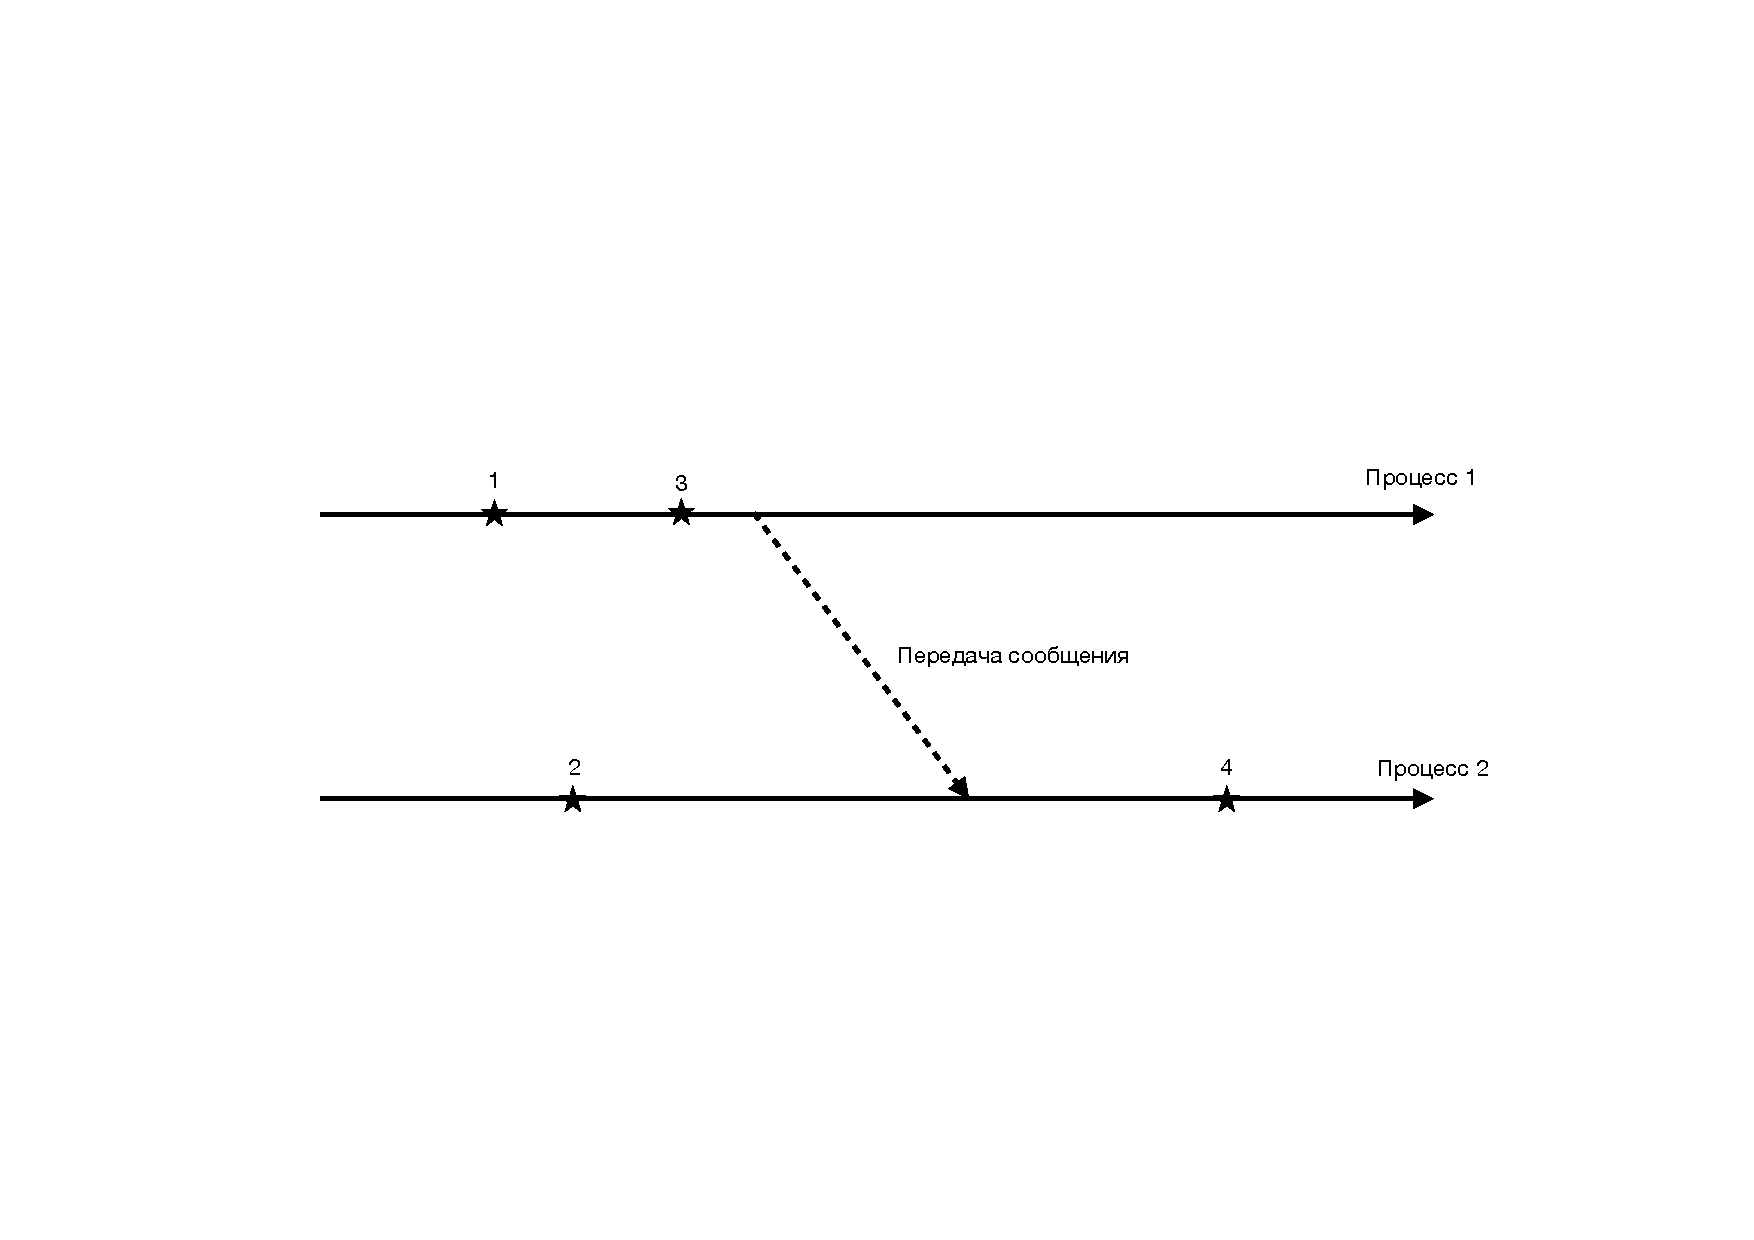
\includegraphics[scale=0.7]{15/masseg_time.pdf}

Так, на картинке, процесс 2 знает порядок временных меток в процессе 1 до передачи сообщения (1 и 3) и знает что они все были до метки 4, но сравнить порядок 1 или 3 с меткой 2 нельзя, так в распределённой системе отсутствуют глобальные часы и сиинхронизировать процессы нельзя.
 
 Более подробно этот пункт разобран в билете 20.
 
\item  Синхронные и асинхронные системы.

В синхронных мы знаем точное время задержки (если пакет не был доставлен за какое-то время, то он не будет доставлен никогда), и знаем время ответа другого узла (выполнения операции).

В асинхронных системах не знаем ничего, модель менее удобная, но более жизненная.
\end{itemize} 
\textbf{\noindent 2. Модели ошибок}

Процесс может работать до какого-то момента, после чего отказать и далее:\\
 \textit{Наблюдаемый отказ}  -  другие участники могут узнать, что он погиб.\\
 \textit{Ненаблюдаемый отказ}  - другие участники не могут узнать, что он погиб.\\
\textit{Потеря} (в канале) - сообщение отправленно, но не дошло. \\
\textit{Пропуск отправки} (в процессе) - не отправляет сообщения.\\
\textit{Пропуск приема} (в процессе) - не получает сообщения.\\
\textit{Произвольное поведение} (и в канале, и в процессе) - поведение, не предписанное протоколом, возникшее из-за ошибок или злоумышленно.\\
\\
\textbf{\noindent 3. Модели безопасности}
\begin{itemize}
\setlength\itemsep{0.0001em}
\item Описание информационной системы
\item Структурно-функциональные характеристики
\item Описание угроз безопасности
\item Модель нарушителя
\item Возможные уязвимости
\item Способы реализации угроз
\item Последствия от нарушения свойств безопасности информации.
\end{itemize}





\newpage
\section {Билет 16. Архитектуры информационных систем: "монолитная", клиент-серверная, многоуровневая. Одноранговые системы (peer-to-peer).}
\newpage
\section{Билет 17. Основные уровни сетевых протоколов. Семиуровневая модель OSI. Сети пакетной коммутации. Маршрутизация сообщений.}\label{b17:part1}

Перейти к~\nameref{b17:part2}

\textbf{Протокол} -- это набор соглашений между разработчиками ПО и аппаратуры. Текст протокола отвечает на вопрос: «Что нужно сделать, чтобы программы и устройства могли взаимодействовать с другими программами/устройствами, поддерживающими протокол».

\href{https://clck.ru/BmJYw}{\textbf{OSI}} (Open Systems Interconnection model) -- открытая сетевая модель.

Модель описывает, какие уровни должны быть в сети и какие функции выполняются на каждом из уровней. OSI модель разделяет все протоколы на 7 таких уровней:
\begin{enumerate}
\item \nameref{b17:osi:lev1} (Physical)
\item \nameref{b17:osi:lev2} (Datalink)
\item \nameref{b17:osi:lev3} (Network)
\item \nameref{b17:osi:lev4} (Transport)
\item \nameref{b17:osi:lev5} (Session)
\item \nameref{b17:osi:lev6} (Presentation)
\item \nameref{b17:osi:lev7} (Application)
\end{enumerate}

Все они отвечают за определенную ступень процесса отправки сетевого сообщения, а также содержат в себе определенную информацию. Шаги выполняются, обособленно друг от друга. Модель OSI \textbf{не включает} описание протоколов; они определяются в отдельных стандартах.

\textbf{Media layers} (уровни 1-3) управляют физической доставкой данных по сети. \\
\textbf{Host layers} (уровни 4-7) способствуют обеспечению точной доставки данных между компьютерами в сети.

\textbf{PDU} (Protocol data unit) -- это информация, доставляемая между одноуровневыми объектами сетей.

\begin{figure}[H] \centering
	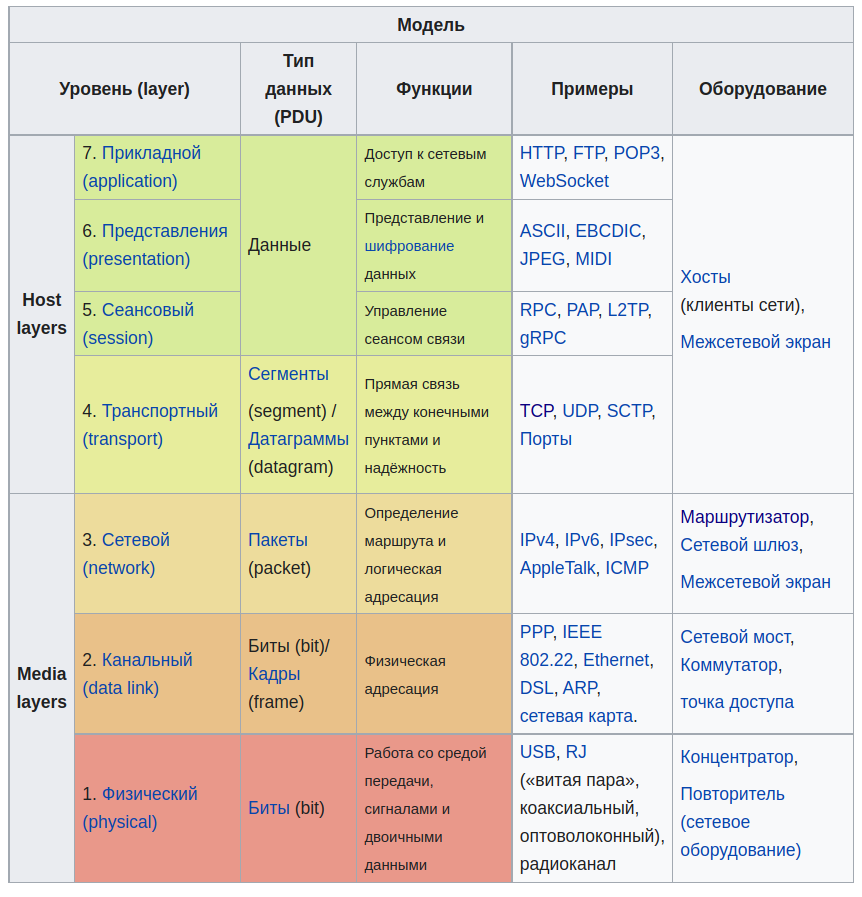
\includegraphics[scale = 0.6]{17/OSI.png}
	\caption{Уровни модели OSI}
\end{figure}

\paragraph*{Физический уровень}\label{b17:osi:lev1} отвечает за обмен физическими сигналами между физическими устройствами. Основная его цель представить нуль и единицу в качестве сигналов, передаваемые по среде передачи данных. Никакой гарантии корректности передачи нет.

\paragraph*{Канальный уровень}\label{b17:osi:lev2} предназначен для обеспечения взаимодействия сетей на физическом уровне и контроля ошибок, которые могут возникнуть. Канальный уровень получает (от физического уровня) биты, находит начало и конец сообщения и упаковывает биты в кадры (фреймы). проверяет их на целостность и, если нужно, исправляет ошибки (либо формирует повторный запрос повреждённого кадра) и отправляет на сетевой уровень. Задача здесь — сформировать кадры с адресом отправителя и получателя, после чего отправить их по сети.

У канального уровня есть два подуровня -- это MAC и LLC. MAC (Media Access Control, контроль доступа к среде) отвечает за присвоение физических MAC-адресов, а LLC (Logical Link Control, контроль логической связи) занимается проверкой и исправлением данных, управляет их передачей.

\paragraph*{Сетевой уровень}\label{b17:osi:lev3} предназначен для определения пути передачи данных. Получает MAC-адрес от коммутаторов с предыдущего уровня и занимаются построением маршрута от одного устройства к другому с учетом всех потенциальных неполадок в сети. Преобразует физический адрес (MAC) в логический (IP).

\paragraph*{Транспортный уровень}\label{b17:osi:lev4} предназначен для обеспечения надёжной передачи данных от отправителя к получателю (т.е. без потерь).

При передаче по протоколу TCP, данные делятся на сегменты. Сегмент -- это часть пакета. Когда приходит пакет данных, который превышает пропускную способность сети, пакет делится на сегменты допустимого размера. Сегментация пакетов также требуется в ненадежных сетях, когда существует большая вероятность того, что большой пакет будет потерян или отправлен не тому адресату.

При передаче данных по протоколу UDP, пакеты данных делятся уже на датаграммы. Датаграмма (datagram) -- это тоже часть пакета, но ее нельзя путать с сегментом. Главное отличие датаграмм в автономности. Каждая датаграмма содержит все необходимые заголовки, чтобы дойти до конечного адресата, поэтому они не зависят от сети, могут доставляться разными маршрутами и в разном порядке.

Датаграмма и сегмент -- это два PDU транспортного уровня модели OSI. При потере датаграмм или сегментов получаются «битые» куски данных, которые не получится корректно обработать.

\paragraph*{Сеансовый уровень}\label{b17:osi:lev5} устанавливает и поддерживает продолжительные соединения, сеансы связи.
Уровень управляет созданием/завершением сеанса, обменом информацией, синхронизацией задач, определением права на передачу данных и поддержанием сеанса в периоды неактивности приложений.
Примером работы пятого уровня может служить видеозвонок по сети. Во время видеосвязи необходимо, чтобы два потока данных (аудио и видео) шли синхронно.

\paragraph*{Представительный уровень}\label{b17:osi:lev6} занимается тем, что представляет данные (которые все еще являются PDU) в понятном человеку и машине виде. Например, когда одно устройство умеет отображать текст только в кодировке ASCII, а другое только в UTF-8, перевод текста из одной кодировки в другую происходит на шестом уровне.
Шестой уровень также занимается представлением картинок (в JPEG, GIF и т.д.), а также видео-аудио (в MPEG, QuickTime). Помимо перечисленного, шестой уровень занимается шифрованием данных, когда при передаче их необходимо защитить.

\paragraph*{Прикладной уровень}\label{b17:osi:lev7} -- это ближайший уровень к пользователю. На нем реализуются протоколы на уровне приложений, такие как HTTP.  Его задача, визуализировать или записать данные, взаимодействовать с пользователем.
\bigskip

\textbf{Инкапсуляция} -- весь процесс преобразования данных (с верхнего уровня) в сигналы (на нижний уровень), обратный ему процесс называется \textbf{декапсуляцией}.

Исторически вышло, что на практике модель взаимодействия открытых систем не применяется. Раньше существовали её буквальные реализации, содержащие ровно 7 слоев. Однако со временем их вытеснил менее предписывающий набор протоколов TCP/IP, на котором построен современный Интернет. Тем не менее, модель OSI до сих пор используется в качестве эталона для обучения и документации.


\subsection*{Сети пакетной коммутации. Маршрутизация сообщений.}\label{b17:part2}

Перейти к~\nameref{b17:part1}

\textbf{Пакетная коммутации} -- процесс передачи пакетов с использованием транзитных узлов.

\textbf{Маршрутизация} -- процесс определения маршрута данных в сетях связи.

Хотим передать большой файл от A к B. Наше сообщение делится на пакеты, в соответствии с используемым протоколом.
А -> роутер -> маршрутизатор.
У одного маршрутизатора есть несколько физических входящих и исходящих каналов. Соответственно на один маршрутизатор могут приходить пакеты с разных узлов. Внутри маршрутизатора своя очередь приема пакетов и соответственно очередь передачи.
Задача маршрутизатора глядя на логические адреса (куда нужно доставить сообщение), выбрать оптимальный маршрут.

Очередь отправки может переполниться. (Лектор говорит, что очередь приёма не переполняется, так как время обработки пакета в маршрутизаторе согласовано с пропускной способностью.) Может случиться, что пакеты пришли с двух узлов, а отправить их маршрутизатор решил дальше по одному каналу -- в этот момент может произойти переполнение.
Маршрутизатору не хватает ресурсов запомнить все пакеты, которые нужно отправить, а пропускной способности соединения не хватает, чтобы отправить эти пакеты. В такой ситуации маршрутизатор может потерять пакет.

Когда передаем сообщение от А к В, это сообщение проходит через какое-то количество промежуточных устройств. Чем больше устройств, тем больше шанс потерять сообщение, тем больше задержка.

Внутри маршрутизатора строятся таблицы маршрутизации -- они помогают определять оптимальный путь сообщения. Так же в случае недоступности узла, спустя время все пути перестраиваются (для ещё не отправленных сообщений).
\newpage
\section{Билет 18. Невозможность гарантированной доставки сообщений. Алгоритм скользящего окна.} \label{b18:part1}

Перейти к~\nameref{b18:part2}

\textbf{Надёжность} -- доставка без потерь и дублирования. \newline
\noindent A, B -- процесс, программа которая выполняется. \newline
\noindent \textbf{NCP} -- Network Control Procedure, управление сетью.

У нас есть взаимодействие между приложением и NCP, между NCP и сетью передачи данных.
Если мы хотим обеспечить «надёжность» передачи данных (в кавычках, потому что реальную надёжность обеспечить невозможно), то между NCP и сетью передачи данных должен быть протокол взаимодействия.

Приложение А отправляет сообщение и забывает о нём, а NCP A взаимодействует с NCP B по ненадёжной сети передачи данных.
У NCP есть два события: \textbf{recieve} (получение) -- из сети передачи данных в NCP пришло сообщение, и \textbf{deliver} (доставка) -- NCP решило что сообщение может быть доставлено процессу.
\newline
\begin{figure}[H] \centering
	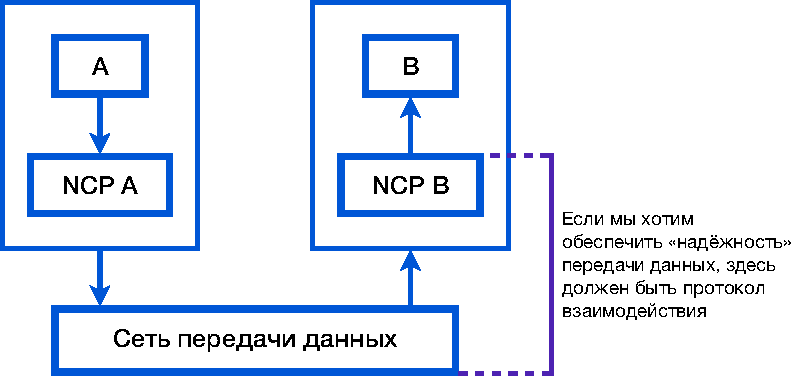
\includegraphics[scale = 1]{18/common.pdf}
\end{figure}

\textbf{\textit{Отличие recieve и deliver}}: в NCP пришёл пакет 2, но не пришел пакет 1 -- событие recieve произошло, но мы не можем отправить пакет 2 в приложение, потому что нарушим порядок -- событие deliver не произошло.

Ненадёжность доставки сводиться к потере пакетов в силу неисправности оборудования или ресурсного ограничения на любом шаге взаимодействия.
\bigskip

Надёжная передача между А и В невозможна, например, если NCP может потерять состояние диалога (перезапуститься).
Пусть NCP B должна доставить процессу B информацию после получения сообщения M от NCP A.
Если NCP B перезапустится после отправки M, то ни один из процессов не может понять было ли доставлено сообщение: у А нет информации, что происходит на стороне B (это удаленная система); так так система со стороны B перезапустилась, то она ничего не помнит.
Повторная передача может привести к дублированию, отказ -- к потере.
\textbf{\textit{Вывод: мы не можем контролировать факт доставки из NCP в процесс.}}

\subsection*{Протоколы, которые передают данные между NCP.}
Рассмотрим разные протоколы общения между NCP. Их можно разделить по количеству сообщений которые передаются.

\textbf{\textit{С 1 сообщением}}: «отправил и забыл» (UDP).

\textbf{\textit{С 2 сообщениями}}: в протокол добавляется подтверждение о получении сообщения -- <\textbf{ack}> (acknowledgment).

\begin{algorithm}
	\caption{Протокол с 2 сообщениями. Нормальный сценарий.}
	\begin{enumerate}
		\item NCP A отправляет <\textbf{data}, m>
		\item NCP B получает <\textbf{data}, m> \\
			доставляет m; отправляет <\textbf{ack}>; закрывает сеанс
		\item NCP A получает <\textbf{ack}> \\
			уведомляет процесс о доставке; закрывает сеанс
	\end{enumerate}
\end{algorithm}

\textbf{DN} (Data network) -- сеть передачи данных.

\begin{algorithm}
	\caption{Протокол с 2 сообщениями. Таймер. Сообщение дублируется.}
	\begin{enumerate}
		\item NCP A отправляет <\textbf{data}, m>
		\item NCP B получает <\textbf{data}, m> \\
			доставляет m; отправляет <\textbf{ack}>; закрывает сеанс
		\item DN Потеря сообщения (<\textbf{ack}>)
		\item NCP A ожидает timeout \\
			убеждается, что к нему не пришло подтверждение и отправляет <\textbf{data}, m>
		\item NCP B получает <\textbf{data}, m> \\
			доставляет m; отправляет <\textbf{ack}>; закрывает сеанс
		\item NCP A получает <\textbf{ack}> \\
			уведомляет процесс о доставке; закрывает сеанс
	\end{enumerate}
\end{algorithm}

\newpage

\textcolor{olive}{Здесь не путать сообщения протокола и те, что отправляем.}\\
В следующем примере, как и в предыдущих, протокол с 2 сообщениями (\textbf{data} + <\textbf{ack}>). И к тому же отправляем 2 сообщения <\textbf{data}, $m_1$> и <\textbf{data}, $m_2$>.

\begin{algorithm}
	\caption{Протокол с 2 сообщениями. Потеря.}
	\begin{enumerate}
		\item NCP A отправляет <\textbf{data}, $m_1$>
		\item NCP B получает <\textbf{data}, $m_1$> \\
			доставляет $m_1$; отправляет <\textbf{ack}>; закрывает сеанс
		\item NCP A ожидает timeout \\
			убеждается, что к нему не пришло подтверждение и отправляет <\textbf{data},  $m_1$>
		\item NCP B получает <\textbf{data},  $m_1$> \\
			доставляет m; отправляет <\textbf{ack}>; закрывает сеанс
		\item NCP A получает <\textbf{ack}> (отправленное на шаге 4) \\
			уведомляет процесс о доставке; закрывает сеанс
		\item NCP A отправляет <\textbf{data}, $m_2$>
		\item DN Потеря сообщения (<\textbf{data}, $m_2$>)
		\item NCP A получает <\textbf{ack}> (отправленное на шаге 2) \\
			уведомляет процесс о доставке; закрывает сеанс
	\end{enumerate}
\end{algorithm}

Получилось, что А получил дважды подтверждение от получении <\textbf{data}, $m_1$>, но с его стороны это выглядело как 2 подтверждения для $m_1$ и $m_2$. Процесс А думает, что передача успешная, а на самом деле B не получил второе сообщение.

\newpage
\textbf{\textit{С 3 сообщениями}}: в протокол хотим добавить подтверждение, что получено подтверждение <\textbf{close}>. Повторная передача при потере <\textbf{data}, m> или <\textbf{ack}>.

\begin{algorithm}
	\caption{Протокол с 3 сообщениями. Нормальный сценарий.}
	\begin{enumerate}
		\item NCP A отправляет <\textbf{data}, m>
		\item NCP B получает <\textbf{data}, m> \\
			доставляет m; отправляет <\textbf{ack}>
		\item NCP A получает <\textbf{ack}> \\
			уведомляет процесс о доставке; отправляет <\textbf{close}>; закрывает сеанс
		\item NCP B получает <\textbf{close}>; закрывает сеанс
	\end{enumerate}
\end{algorithm}

\begin{algorithm}[h!]
	\caption{Протокол с 3 сообщениями. Потеря.}
	\begin{enumerate}
		\item NCP A отправляет <\textbf{data}, $m_1$>
		\item NCP B получает <\textbf{data}, $m_1$> \\
			доставляет $m_1$; отправляет <\textbf{ack}>
		\item NCP A получает <\textbf{ack}> \\
			уведомляет процесс о доставке; отправляет <\textbf{close}>; закрывает сеанс
		\item DN потеря сообщения (<\textbf{close}>)
		\item NCP A отправляет <\textbf{data}, $m_2$>
		\item DN потеря сообщения (<\textbf{data}, $m_2$>)
		\item NCP B ожидает timeout (ждет ответа от A, после шага 2) \\
			убеждается, что к нему не пришло подтверждение  и отправляет <\textbf{ack}>
		\item NCP A получает <\textbf{ack}> \\
			уведомляет процесс о доставке; <\textbf{close}>; закрывает сеанс
		\item NCP B получает <\textbf{close}>; закрывает сеанс
	\end{enumerate}
\end{algorithm}


Получилось, что B отправил повторный <\textbf{ack}>, так как не получил от А  <\textbf{close}>. Процесс А думает, что это были 2 подтверждения на получение сообщений $m_1$ и $m_2$. Хотя на самом деле B не получил второе сообщение.

\subsection*{Алгоритм скользящего окна.}\label{b18:part2}

Перейти к~\nameref{b18:part1}

\href{https://www.youtube.com/watch?v=hd6QNXK5rPk}{Хорошее видео на эту тему.}

Ранее рассмотренные протоколы, после отправки ждут подтверждения. Скользящее окно применяется в протоколе TCP.

Концепция \textbf{скользящего окна} (sliding window) заключается в том, что для повышения скорости передачи данных отправителю разрешается передать некоторое количество сообщений, не дожидаясь прихода на эти пакеты подтверждения.

\begin{figure}[H] \centering
	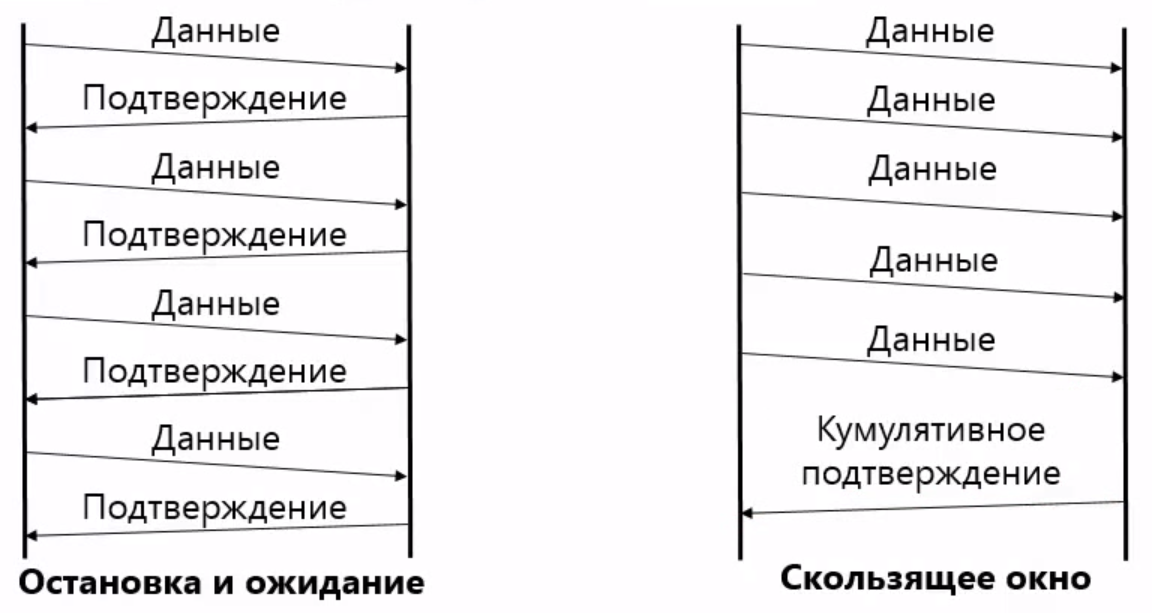
\includegraphics[scale = 0.35]{18/send_types.png}
	\caption{Схематичное различие ранее рассмотренных протоколов и алгоритма скользящего окна}
\end{figure}

\textbf{Размер скользящего окна} -- количество сообщений, которые могут быть отправлены без подтверждения. \\
В примере будет окно размера 8. Без подтверждения можем отправить 8 сообщений.
\begin{figure}[H] \centering
	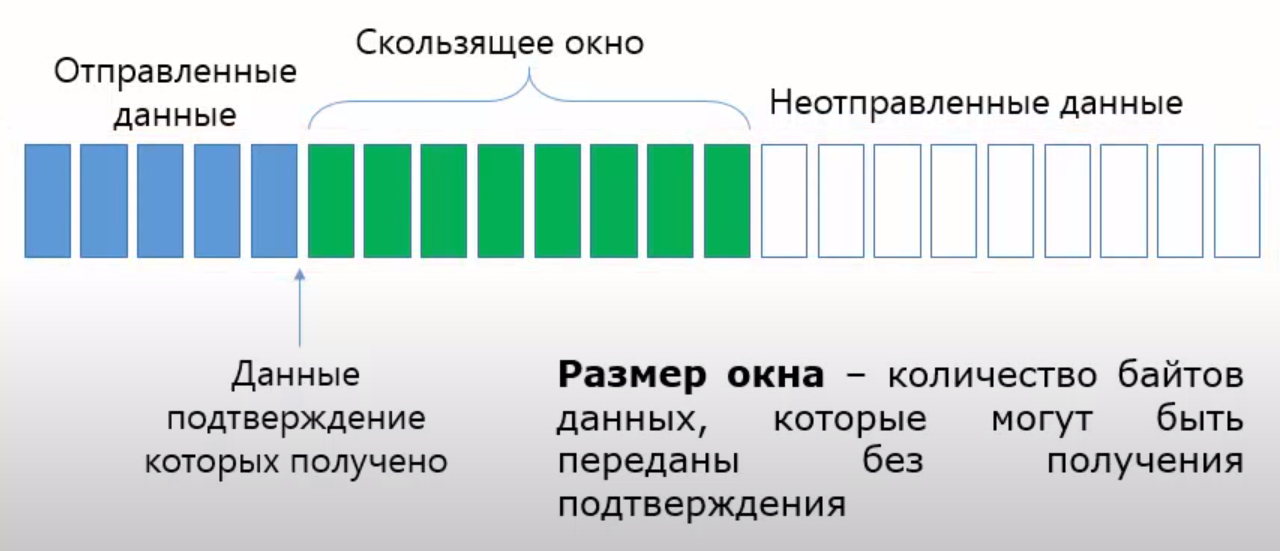
\includegraphics[scale = 0.3]{18/window_1.png}
\end{figure}

Получили часть подтверждений на ранее отправленные данные -- сдвигаем окно на количество полученных подтверждений и отправляем новую порцию данных. В примере получили 3 подтверждения, сдвинули окно на 3, отправили ещё 3 сообщения. После этого отправитель ожидает подтверждения.


\begin{figure}[H] \centering
	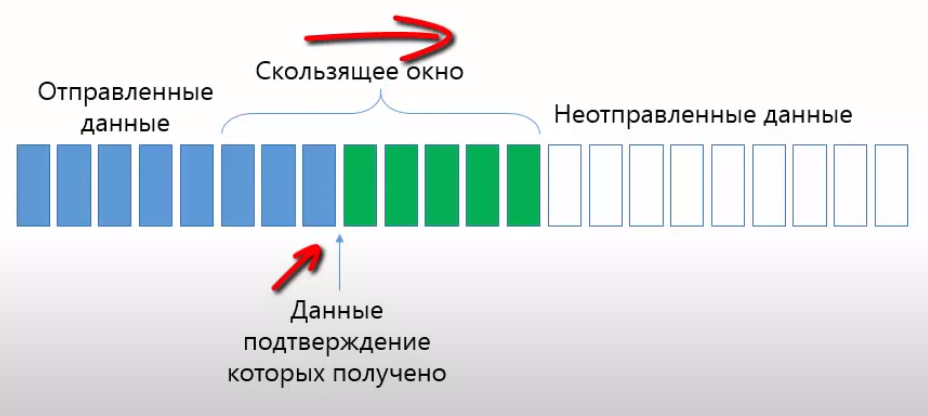
\includegraphics[scale = 0.4]{18/window_2.png}
	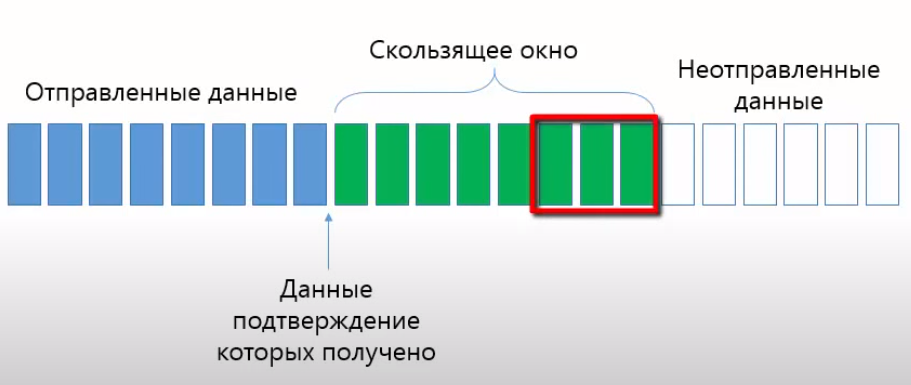
\includegraphics[scale = 0.4]{18/window_3.png}
	\caption{Сдвиг окна}
\end{figure}

\newpage
\section{Билет 19. Многоадресная передача. Протоколы B-, R-, CO-, ТО-multicast: устойчивость к сбоям, сложность по числу сообщений и времени.}

Ранее рассматриваемые проколы были по типу «точка-точка».
Теперь некоторое множество процессов объединены в группы, и внутри этой группы необходимо организовать передачу сообщений.

\textbf{Задача}: передать сообщения всем участникам (закрытой) группы (с выполнением некоторых дополнительных условий).

Мы знаем всех участников группы. $N$ -- количество процессов в группе. Будем считать, что процессы могут только падать.
Корректный процесс никогда не падает, некорректный -- до какого-то момента работает, падает и не перезапускается.

\textbf{Условие надежности} -- если один корректный процесс сообщение получил, то все остальные корректные процессы сообщение тоже получат.
\bigskip

Протоколы многоадресной передачи:
\begin{itemize}
	\item B-multicast (Basic)~\ref{b19:part1}
	\item R-multicast (Reliable -- надежность)~\ref{b19:part2}
	\item FIFO-multicast (первым пришёл -- первым ушёл)~\ref{b19:part3}
	\item TO-multicast (Total ordering -- глобальный порядок)~\ref{b19:part4}
	\item CO-multicast (Causal ordering -- отношение причинно-следственной зависимости)~\ref{b19:part5}
\end{itemize}

\newpage
\subsection*{B-multicast}\label{b19:part1}

\begin{algorithm}[h!]
\caption{B-multicast. Примитивы.}
\begin{algorithmic}
\algtext*{EndProcedure}
%\let\algorithmicprocedure=\relax \algtext*{EndFor}

\State Процесс $p$ посылает сообщение $m$ в группу $G$
\Procedure{B-multicast}{$m$, $G$}:
	\For{$q$ in $G$}:
		\State send($m$, $q$)
	\EndFor
\EndProcedure
\State
\State Получили в процессе $p$ сообщение $m$ от процесса $q$
\Procedure{B-recieve}{$m$, $q$}:
	\State B-deliver($m$) -- передать сообщение $m$ в свой процесс
\EndProcedure

\end{algorithmic}
\end{algorithm}

\textbf{B-multicast не гарантирует надежность.} Пример: \\
Процесс $p$ -- некорректный, отправляет всем сообщения, но ломается. Пусть успел отправить только процессу $q$, который оказался корректным. И кроме $q$ в группе есть ещё корректные процессы, тогда условие надежности не выполнено.

Отправим $N$ сообщений. Сообщение будет доставлено за время одной передачи.


\subsection*{R-multicast}\label{b19:part2}

\begin{algorithm}
\caption{R-multicast. Примитивы.}
\begin{algorithmic}
\algtext*{EndProcedure}

\State Процесс $p$ посылает сообщение $m$ в группу $G$
\Procedure{R-multicast}{$m$, $G$}:
	\State B-multicast($m$, $G$)
\EndProcedure
\State
\State Получили в процессе $p$ сообщение $m$ от процесса $q$
\Procedure{R-recieve}{$m$, $q$}:
	\If{$m$ not in $M$}
		\State R-deliver($m$) -- передать сообщение $m$ в свой процесс
		\State B-multicast($m$, $G$)
		\State $M += m$ -- запоминаем какие сообщения получили
	\EndIf
\EndProcedure

\end{algorithmic}
\end{algorithm}

Проблемы, описанной для B-multicast, в R-multicast не возникает. \\
Отправим $N^2$ сообщений. Сообщение будет доставлено за время одной передачи.

\newpage
\subsection*{FIFO-multicast}\label{b19:part3}

\begin{algorithm}
\caption{FIFO-multicast. Примитивы.}
\begin{algorithmic}
\algtext*{EndProcedure}

\State В каждом процессе $p$ есть локальный счётчик, который нумерует пакеты.
\State $seq_p = [0, \cdot, 0]$ -- вектор размера $N$ -- порядковые номера сообщения отправителя.
\State
\State Процесс $p$ посылает сообщение $m$ в группу $G$
\Procedure{FIFO-multicast}{$m$, $G$}:
	\State $seq_p[p] += 1$
	\State R-multicast(<$seq_p[p]$, $m$>, $G$)
\EndProcedure
\State
\State Получили в процессе $p$ сообщение $m$ от процесса $q$
\Procedure{FIFO-recieve}{<$seq$, $m$>, $q$}:
	\If{$seq == seq_p[q] + 1$}
		\State // Это следующее сообщение, которое мы хотим получить от процесса $q$
		\State FIFO-deliver($m$) -- передать сообщение $m$ в свой процесс
		\State $seq_p[q] = seq$
		Проверить возможность доставки из очереди
	\Else
		\State Поставить в очередь
		\State Проверить возможность доставки
	\EndIf
\EndProcedure

\end{algorithmic}
\end{algorithm}

Сообщения от одного отправителя приходят в том порядке, в котором их послал этот отправитель, то есть от разных отправителей сообщения могут перемешаться.



\subsection*{TO-multicast}\label{b19:part4}

Все процессы должны получать сообщения в одинаковом порядке.

Есть выделенный процесс-нумератор (выбор лидера см.~\ref{b21}), к которому каждый процесс обращается, чтобы получить глобальный порядковый номер своего сообщения.

Процесс $p$ посылает запрос нумератору на получение глобального номера $seq$, и после этого рассылает сообщение всем процессам. Получатели делают очередь -- «глобальный FIFO».

Недостаток: увеличили время на отправку сообщения. Теперь сообщение отправится за 3 передачи (запрос нумератору, ответ нумератора, сама посылка сообщения).

В случае если нумератор упал, мы должны выбрать нового лидера.


\subsection*{CO-multicast}\label{b19:part5}

Хотим задать на множестве событий порядок, события могут быть сравнимы или нет. Сравнимы события в одном процессе -- у нас есть локальные счётчики. Между процессами, мы знаем, что логически отправка сообщения предшествует получению. Подробнее про сравнения см.~\ref{b20}.

Очередь в CO-multicast основана на идеи, что мы не можем пришедшее сообщение доставить в процесс до тех пор, пока мы не получили все сообщения \textbf{логически} предшествующие тому, что стоит в очереди.
\newpage
\section{Билет 20. Отношение причинно-следственной зависимости. Метки Лэмпорта, векторные часы.}\label{b20}
\begin{center}
    \textit{\underline{Отношение причинно-следственной зависимости.}}
\end{center}
 Отношение причинно-следственной зависимости\footnote{Подробнее см. 66 с. книги «Ж. Тель. Введение в распределенные алгоритмы. М.: МЦНМО, 2009. — 616 с. — ISBN 978-5-94057-515-3.»} - это аналог понятия  «Справедливости». Можно сравнивать события и узнавать, какое из них произошло раньше, а какое позже. \\ 
Пусть в предположении у нас задано следующее:
\begin{itemize}
\item Сравнимы события в одном процессе (например, с помощью локального счётчика).
\item Сравнимы отправка и получение сообщений. (Отправка сообщения логически предшествует получению этого же самого сообщения.)
\end{itemize}
%Представляя выполнение в виде последовательности переходов, мы тем самым естественно привносим в модель понятие времени. Будем говорить, что переход $a$ происходит раньше, чем переход $b$, если в последовательности переходов событие $a$ предшествует событию $b$.\\
Хотим реализовать механизм сравнения двух событий в случае, если они сравнимы.\footnote{Узнать что произошло раньше, а что позже (транзитивное замыкание описанных двух отношений).}

Пусть $n$ - количество процессов. $\forall p = 1, \ldots, n$ заводим свой счётчик $L_p := 0;$ событий.\\
Внутри процесса могут происходить локальные события, которые мы хотим учесть при общем сравнении, поэтому мы их тоже будем помечать. (см. \nameref{algComparison})

\begin{algorithm}
\caption{Алгоритм сравнения событий. Метки Лэмпорта}
\label{algComparison}
\begin{algorithmic}
\State $L_p \gets 0$
\Function{matching}{$e$}\Comment{Приписываем событию $e$ временную метку $L(e)$ (Leslie Lamport).}
%\State 
\If{$e$ - локальное событие в процессе $p$}
    \State $L_p += 1$
    \State $L(e) \gets L_p$ \Comment{Нумеруем локальное событие своим же счётчиком.}
\EndIf
\If{$e$ - отправка сообщения $message$ процессу $q$ от процесса $p$}
    \State $L_p += 1$
    \State $send(<message, L_p>, q)$ \Comment{Вместе с данными передаём свою метку времени.}
\EndIf
\If{$e$ - получение сообщения $<message, L>$ от процесса $q$ в  процессе $p$}
    \State $L_p \gets \max\{L,L_p\} + 1$
    \State $L(e) \gets L_p$ \Comment{Получение сообщения тоже может быть учтено как событие $e$.}
\EndIf
\EndFunction
\end{algorithmic}
\end{algorithm}

%Приписываем событию $e$ временную метку $L(e)$ (Leslie Lamport).\\ \\
%Когда происходит локальное событие $e$ в процессе с номером $p$:\\
%\ \ \ \ $L_p += 1;$\\
%\ \ \ \ $L(e) = L_p;$ //Нумеруем локальное событие своим же счётчиком. \\ \\ 
%Отправка сообщения $message$ процессу с номером $q$ от процесса с номером $p$:\\
%\ \ \ \ $L_p += 1;$\\
%\ \ \ \ $send(<message, L_p>, q);$ //Вместе с передаваемыми данными передаём свою метку времени.\\ \\
%Получение сообщения $<message, L>$ от процесса с номером $q$ в  процессе с номером $p$:\\ 
%\ \ \ \ $L_p = \max\{L,L_p\} + 1;$\\
%\ \ \ \ $L(e) = L_p;$ //Получение сообщения тоже может быть учтено как событие $e$. \\

\textbf{Итого:} У всех исходно нулевой счётчик. Каждому событию, которое мы хотим сравнивать, приписываем числовую временную метку. Для локальных событий в $p$ увеличиваем локальный счётчик на $1$. Отправляя сообщение, локально подписываем факт отправки и затем отправляем свою метку. Получая сообщение, вычисляем максимум временных меток.

Пусть событие $e_1$ произошло точно раньше события $e_2$ по нашему заданному отношению причинно-следственной зависимости (либо произошли в одном процессе и $e_1$ раньше $e_2$, либо в разных, но между ними $\exists$ цепочка попарно-сравнимых событий).
Тогда $L(e_1) < L(e_2)$. (По построению будет так)

\textbf{Замечание:} Обратное неверно! (См. рисунок. \ref{fig:Image_comparsion})

\begin{figure}[H]
\center{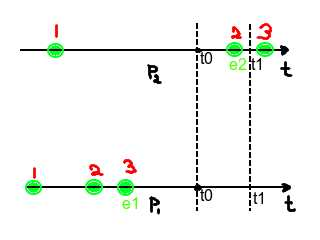
\includegraphics[width=0.9\textwidth]{20/Comparison_for_labels.jpg}}
\caption{В момент $t_0$: $2 = L_{p_2} < L_{p_1} = 3$, хотя событие $e_1 < e_2$.} 
\label{fig:Image_comparsion}
\end{figure}
        
Для выполнения необходимого и достаточного условия ($e_1 < e_2 \Leftrightarrow L(e_1) < L(e_2)$) реализуют механизм под названием «векторные часы». Разница с предыдущим алгоритмом лишь в том, что во всех процессах ведётся учёт временных меток не одного процесса, а целого вектора (массива) временных меток $\bar{L}_p := (L_p^1, \ldots, L_p^n)^T$ всех процессов.
Приведём \nameref{algComparisonVecClock}.
\begin{algorithm}
\caption{Алгоритм сравнения событий. Векторные часы}
\label{algComparisonVecClock}
\begin{algorithmic}
\State $L_p \gets (\underbrace{0,\ldots,0}_{n}) = \bar{0}$
\Function{matching}{$e$} \Comment{Приписываем событию $e$ временную метку $L(e)$ (Leslie Lamport).}
\If{$e$ - локальное событие в процессе $p$}
    \State $L_p[p] += 1$
    \State $L(e) \gets L_p$ \Comment{Нумеруем локальное событие своим же счётчиком.}
\EndIf
\If{$e$ - отправка сообщения $message$ процессу $q$ от процесса $p$}
    \State $L_p[p] += 1$
    \State $send(<message, L_p>, q)$ \Comment{Вместе с данными передаём свою метку времени.}
\EndIf
\If{$e$ - получение сообщения $<message, L>$ от процесса $q$ в  процессе $p$}
    \For{$i = 1, \ldots, n$}
        \State $L_p[i] \gets \max\{L[i],L_p[i]\}$
    \EndFor
    \State $L_p[p] += 1$
    \State $L(e) \gets L_p$\Comment{Получение сообщения тоже может быть учтено как событие $e$.}
\EndIf
\EndFunction
\end{algorithmic}
\end{algorithm}
%$\forall p = 1, \ldots, n$ заводим свой массив счётчиков $\bar{L}_p := \bar{0};$ событий.\\ \\
%Когда происходит локальное событие $e$ в процессе с номером $p$:\\
%\ \ \ \ $L_p[p] += 1;$\\
%\ \ \ \ $L(e) = L_p;$ //Нумеруем локальное событие своим же счётчиком. \\ \\
%Отправка сообщения $message$ процессу с номером $q$ от процесса с номером $p$:\\
%\ \ \ \ $L_p[p] += 1;$\\
%\ \ \ \ $send(<message, L_p>, q);$ //Вместе с передаваемыми данными передаём свою метку времени.\\ \\
%Получение сообщения $<message, L>$ от процесса с номером $q$ в  процессе с номером $p$:\\
%\ \ \ \ $L_p[i] = \max\{L[i],L_p[i]\};\ \forall i = 1, \ldots, n.$\\
%\ \ \ \ $L_p[p] += 1;$\\
%\ \ \ \ $L(e) = L_p;$ //Получение сообщения тоже может быть учтено как событие $e$.\\

Итого: $e_1 < e_2 \Leftrightarrow L(e_1)[i] \leq L(e_2)[i]\ \forall i = 1,\ldots, n$ покоординатно, причём $\exists i: L(e_1)[i] < L(e_2)[i]$ строго.

Если $\exists i_1, i_2 \in [1,n]: L(e_1)[i_1]< L(e_2)[i_1]$ и при этом же $L(e_1)[i_2] >  L(e_2)[i_2] $, то события $e_1$ и $e_2$ не сравнимы.

\textbf{Замечание:} Multicast, построенный на основе векторных часов - это CO-multicast. (Не можем доставить пришедшее сообщение в процесс до тех пор, пока не получили все сообщения, логически предшествующие тому, что стоит в  очереди.)

\newpage
\section{Билет 21. Алгоритмы избрания лидера. Свойства завершения, единственности и согласия. Выборы в кольцевой сети. Выборы на основе протоколов многоадресной передачи. Справедливость.}\label{b21}
\textbf{Задача избрания лидера.}\\
Исходные предположения постановки задачи:
\begin{itemize}
\item Все процессы, которые объединены в нашей системе, выполняют один и тот же алгоритм (т.е. они однородны).
\item Сам алгоритм может запускаться одновременно несколькими процессами.
\item В момент завершения алгоритма ровно один процесс находится в выделенном состоянии лидера. (Ни в какой момент не бывает двух лидеров, а также их может временно не быть вообще.)
\end{itemize}

Примеры задач избрания лидера: 
\begin{itemize}
\item Выбор ведущего сервера, который будет обрабатывать запросы;
\item В многоадресовой передаче выбрать процесс, отвечающий за нумерацию сообщений.
\end{itemize}

Варианты задачи определяются из практических соображений, поэтому имеем различные предположения:
\begin{itemize}
\item Синхронная или асинхронная система;
\item Знаем ли верхнюю границу на время передачи/обработки сообщений или нет;
\item Есть ли у процессов их идентификаторы (упорядоченные);
\item Надёжность сети: пропадают сообщения или нет;
\item Различные топологии сети.
\end{itemize}

\textbf{Выбор в кольцевых сетях.}\\
Требования:
\begin{enumerate}
\item Топология сети - кольцо;
\item У каждого процесса есть сосед справа. Только ему можно передавать сообщения;
\item У каждого процесса есть уникальный идентификатор и он сам его знает;
\item Нет никаких потерь;
\item Канал связи между соседями надёжен и обеспечивает очерёдность доставки FIFO (Сообщение отправленное первым - доставится первым);
\item Система асинхронна(нет предположений на время работы).
\end{enumerate}

\begin{algorithm}
\caption{Алгоритм выбора в кольцевых сетях. LeLann(1977)}
\label{algLeLann}
\begin{algorithmic}
\State Идея алгоритма в том, что все процессы сначала хотят составить список всех кандидатов, а потом применить процедуру выбора. Кто победил - лидер. 
\Require $n$ - количество процессов, Исходно все процессы - спят. $Prev(p), Next(p)$ - номера соседей слева, справа соответственно.
\Ensure $state_p$\\
$List_p:=\{p\}_{p=1}^n$ \Comment{Список всех известных процессу идентификаторов.}\\ 
$state_p \in \{sleep, lost\text{(Проиграл)}, leader, cand\text{(Кандидат)}\}$ \Comment{список состояний.}
\If{$p$ - инициатор} \Comment{Просыпается один - устраивает выбор лидера.}
    \State $State_p \gets cand$
    \State $send(<message, p>, Next(p))$ \Comment{Посылаем сообщение соседу справа.}
    \State $recv(<message, q>, Prev(p))$ \Comment{Ждём от соседа слева сообщения.}
    \While{$q \neq p$} \Comment{Значит в кольце кто-то ещё захотел стать лидером.}
        \State $List_p \gets List_p \cup {q}$
        \State $send(<message, p>, Next(p))$ \Comment{Передаём дальше, чтобы все остальные сформировали тот же список кандидатов.}
        \State $recv(<message, q>, Prev(p))$ \Comment{Ждём от соседа слева сообщения.}
        \State //Как только $q = p$, значит сообщение сделало полный оборот.
    \EndWhile
    \If{$p = \min(List_p)$} \Comment{Какая-нибудь функция выбора лидера.}
        \State $State_p \gets leader$
    \Else 
        \State $State_p \gets lost$
    \EndIf
    \State В этот момент можно запустить алгоритм оповещения всех о том, кто победил.
\Else[Не инициаторы] \Comment{Выступает в роли посредника, пересылая сообщение дальше.}
    \While{$True$}
        \State $recv(<message, q>, Prev(p))$ \Comment{Получают сообщение от кого-то.}
        \State $send(<message, q>, Next(p))$ \Comment{Пересылаем следующему.}
        \If{$state_p = sleep$}
            \State $state_p \gets lost$
        \EndIf
    \EndWhile
\EndIf 
\end{algorithmic}
\end{algorithm}
\nameref{algLeLann} требует $O(n^2)$ переданных сообщений в худшем случае, когда все - кандидаты, а также $O(n)$ времени, чтобы выбрать лидера, в том же случае.

Улучшить \textbf{время работы} нельзя, так как мы должны всё равно всем отправить сообщения, что выбрали лидера, и получить сообщение о том, что никто другой не является ининциатором.

Можно ли уменьшить \textbf{число сообщений}? Да, если получая сообщения, проводить турнир по выбору лидера не глобально после сбора всех кандидатов, а локально, передавая дальше только победителя. См. \nameref{algRoberts}. В этом алгоритме сообщений в среднем $O(n\log n)$. В худшем $O(n^2)$.
\begin{algorithm}
\caption{Алгоритм выбора в кольцевых сетях. Chang-Roberts(1979)}
\label{algRoberts}
\begin{algorithmic}
\State Теперь нам больше не нужен список кандидатов $List_p$. Идея алгоритма в том, что мы сразу выкидываем кандидатов, которые проигрывают.
\State $state_p \in \{sleep, lost\text{(Проиграл)}, leader, cand\text{(Кандидат)}\}$ \Comment{список состояний.}
\If{$p$ - инициатор}
    \State $State_p \gets cand$
    \State $send(<message, p>, Next(p))$ \Comment{Посылаем сообщение соседу справа.}
    \While{$state_p \neq leader$} 
        \State $recv(<message, q>, Prev(p))$ \Comment{Ждём от соседа слева сообщения.}
        \If{$q = p$}
            $state_p \gets leader$
        \ElsIf{$q < p$} \Comment{Проиграли выбором по меньшему индексу.}
            \If{$state_p = cand$}
                \State $state_p \gets lost$
                \State $send(<message, q>, Next(p))$
            \EndIf
        \EndIf
    \EndWhile
\Else[Не инициаторы] \Comment{Выступает в роли посредника, пересылая сообщение дальше.}
    \While{$True$}
        \State $recv(<message, q>, Prev(p))$ \Comment{Получают сообщение от кого-то.}
        \State $send(<message, q>, Next(p))$ \Comment{Пересылаем следующему.}
        \If{$state_p = sleep$}
            \State $state_p \gets lost$
        \EndIf
    \EndWhile
\EndIf 
\end{algorithmic}
\end{algorithm}

Можно ли сделать всё-таки $O(n\log n)$ в худшем случае? Да, если кольцо имитирует двунаправленное с помощью нескольких разных типов сообщений. (См. \nameref{algPeterson})
\begin{algorithm}
\caption{Алгоритм выбора в "двунаправленных" кольцевых сетях. Peterson(1982)}
\label{algPeterson}
\begin{algorithmic}
\State Активные процессы - участвуют в выборах, пассивные передают информацию. 
\State $state_p \in \{active, passive, lost\text{(Проиграл)}, leader\}$ \Comment{список состояний.}
\State $state_p \gets passive$
\State $win_p \gets undefined$ \Comment{Номер победителя.}
\State $ci_p \gets p$ \Comment{Самое лучшее значение, которое сейчас известно процессу $p$.}
\State $acn_p$ \Comment{Значение от его соседа.}
\If{$p$ - инициатор}
    \State $State_p \gets active$
\Else 
    \State $State_p \gets passive$
\EndIf
\While{$win_p = undefined$}
    \State $send(<one, ci_p>, Next(p))$ \Comment{Посылаем сообщение типа $one$ соседу справа.}
    \State $recv(<one, q>, Prev(p))$
    \State $acn_p = q$
    \If{$acn_p = ci_p$} \Comment{УСПЕХ!}
        \State $send(<small, ci_p>, Next(p))$ \Comment{Посылаем всем лидера.}
        \State $recv(<small, q>, Prev(p))$ \Comment{Получаем тот же номер, что и отправили. Сделали полный оборот и все признали наше лидерство.}
        \State $win_p \gets acn_p$
    \Else \Comment{Передаём дальше.}
        \State $send(<two, acn_p>, Next(p))$
        \State $recv(<two, q>, Prev(p))$
        \If{$acn_p < ci_p \&\& acn_p < q$} \Comment{Здесь $acn_p$ - полученное на прошлом шаге значение соседа слева.}
            \State $ci_p \gets acn_p$
        \Else 
            \State $state_p \gets passive$ \Comment{Наше $ci_p$ кто-то перебил}
        \EndIf
    \EndIf
\EndWhile
\If{$p$ - пассивный} 
    \State // Передаём информацию дальше.
\EndIf
\State Когда приходит сообщение типа $small$ мы помечаем, что выбрали лидера.
\end{algorithmic}
\end{algorithm}

Как происходит выбор лидера, если нет идентификатора процесса? Вся сеть абсолютно однородная.

В этом случае не существует алгоритма детерминированного выбора лидера, так как алгоритм выполняет одни и те же действия и конфигурация, в которой находится система, симметрична.

Если все стали инициаторами выбора одновременно, то все процессы пошлют все свои сообщения одновременно, а затем получат все сообщения одновременно и примут детерминированное решение одновременно. Тогда они могут вообще ничем не отличаться. Всегда можно найти пример начального состояния, когда лидерами станут все, что запрещено в исходной постановке задачи. Поэтому наша цель - нарушить симметрию между процессами.

\textbf{Алгоритмы со случайным выбором.}(Вероятностные)\\
Идея в том, что каждый активный процесс, который хочет участвовать в выборе лидера, назначет себе идентификатор некоторым случайным образом.
Проблема только в том, что два процесса могут получить один и тот же случайный номер. Тогда в условии равенства номера процесса своему можно нарваться на тот же самый номер, пришедший от другого процесса.

Если известно количество  процессов - $n$, то можно передавать в дополнение к сообщению число $n$ и при каждой передаче уменьшать его на $1$. Тогда в конце убедиться, что при совпадении индексов никого не нашлось другого с тем же номером, можно по равенству $n = 1$, так как если $n > 1$, то полный оборот круга не завершился.

Если $n$ не знаем, то можно передавать счётчик соседям, но начинатья он будет с $0$ и каждый будет прибавлять единицу. Тогда наш процесс получит слева свой номер процесса и некоторое значение запущенного счётчика (пусть $n_0$). $n_0$ - это может быть длина кольца, а может быть расстояние до ближайшего процесса, у которого оказался случано тот же самый номер. Тогда дальше мы отправляем с сообщением второго типа $n_0$ и новый счётчик $k$, начинающийся с $0$, который итерируется в каждом узле круга. Если пришедшее сообщение второго типа $<n_0, k>$ такое, что $n_0 = k$, то мы сделали полный оборот. Единственная проблема, если узлы с одинаковым идентификатором в круге находятся на одинаковом расстоянии друг от друга. (Каждый узел с таким номером, что $n \% R == 0$, где $R$ - расстояние (количество узлов) между узлами с одинаковыми номерами, получит  сообщение, где $<n_0, k>$ таковы, что $n_0 = k$)

Эту проблему нельзя решить. Поэтому мы получаем алгоритм со свойством, что он всегда заканчивает работу, но иногда некорректно, когда несколько процессов выбрали себя в качестве лидеров.

\textbf{Справедливость.}\\
Про неё не было рассказано для алгоритмов выбора лидера, но по аналогии с задачей разделения критической секции можно предположить, что требование справедливости - это требование, чтобы лидера не захватывал всегда только один процесс, а обеспечивалось какое-то справедливое или, по-другому, приблизительно равномерное распределение.

\newpage
\section {Билет 22. Взаимное исключение. Решение на основе сервера. Алгоритм Дейкстры с общими регистрами. Алгоритм Петерсона для двух процессов. Алгоритм на основе голосования (Maekawa).}
\textbf{Взаимное исключение}.

Постановка задачи: \\
Задано N процессов, конкурирующих за \textbf{общий} ресурс. Каждый процесс циклически выполняет код, принадлежащий \textbf{критической секции} (CS), и не принадлежащий ей (т.е. иногда процесс заходит в критическую секцию и потом из неё выходит).
Задача стоит в разработке алгоритма, который гарантирует, что в каждый момент времени в критической секции находится не более одного процесса.

Требования: \\
Основные:
\begin{itemize}
\item \textbf{Safety}: Не более одного процесса находится в критической секции
\item \textbf{Liveness}: Если один или несколько процессов хотят зайти в CS, то рано или поздно по крайней мере один из них зайдет в критическую секцию (при условии, что время нахождения процессов в CS ограничено)
\end{itemize}
Дополнительные:
\begin{itemize}
\item \textbf{Отсутствие голодания}: Если процесс p хочет войти в критическую секцию, то рано или поздно он войдет в критическую секцию \footnote{\textit{прим. авт.:} из Liveness это условие не следует} 
\item \textbf{Справедливость}: Если процесс p захотел зайти в CS раньше процесса q, то он зайдет в неё раньше
\end{itemize}

Задача ставится не только для систем с распределенной памятью, но и для систем с общей памятью: процессы могут взаимодействовать через общие переменные; атомарны только операции чтения или записи.

\nameref{algServer} сначала вызывается алгоритм выбора лидера и выбирается один процесс лидер $seq$
Далее для всех процессов кроме лидера будет один алгоритм, для лидера другой. Данный алгоритм не удовлетворяет условию справедливости

\begin{algorithm}
\caption{Решение на основе сервера}
\label{algServer}
\begin{algorithmic}
\State У процессов, которые не являются лидерами есть два метода:
\Procedure{try:}{} \Comment{попытка входа в CS}
  \State send (seq, <enter, i>) \Comment{seq - идентификатор лидера, i - номер запрашивающего процесса} 
  \State wait (<allow>) \Comment{i-ый процесс ждёт разрешения}
  \State IN CS \Comment{попал в критическую секцию}
\EndProcedure

\Procedure{exit:}{} 
  \State send (seq, <exit, i>) 
\EndProcedure
\\
\State Лидер должен уметь обрабатывать запросы, которые к нему приходят:
\Procedure{init:}{}  \Comment{запуск сервера}
  \State queue = []
  \State current = None \Comment{CS свободна}
\EndProcedure

\Procedure{on}{<enter, i>} \Comment{обработка запроса на вход в CS}
  \If{current == None}
    \State send (i, <allow>) 
  \Else
    \State queue += i
  \EndIf  
\EndProcedure

\Procedure{on}{<exit, i>}  \Comment{обработка запроса на выход из CS}
  \If{queue is not empthy}
    \State q = queue.getFirst ()
    \State current = q
    \State send (q, <allow>)
  \Else
     \State current = None
  \EndIf
\EndProcedure


\end{algorithmic}
\end{algorithm}

\begin{algorithm}
\caption{Алгоритм Деккера}
Решение задачи взаимного исключения для двух процессов: 
\label{algDekker}
\begin{algorithmic}
\Ensure \\$status[2]$ \Comment{массив из двух чисел. Для чтения каждому из процессов. Для записи у $i$-ого процесса есть доступ только к $i$ ячейке.}\\ 
$turn$ \Comment{переменная, в которую оба процесса могут записывать и читать данные}\\ 
\While{$status[other] == competing$} 
  \If{$turn == other$} 
    \State $status[i] = out$
    \State $wait until (turn == i)$
    \State $status[i] = competing$
  \EndIf
\EndWhile

\State \textbf{CS}
\State $turn = other$
\State $status[i] = out$
\end{algorithmic}
\end{algorithm}


\begin{algorithm}
\caption{Алгоритм Дейкстры}
Решение задачи взаимного исключения для N процессов: 
\label{algDijkstra}
\begin{algorithmic}
\Ensure \\$status[i] \in \{competing, out, cs\}$ \\
$turn \in \{1,...N\}$ 

\Repeat
  \While{$turn \neq i$} 

    \If{$status[turn] == out$} 
      \State $turn := i$
    \EndIf
  \EndWhile
  \State $status[i] = cs$
\Until{$\nexists other:\ status[other] = cs$}
\State \textbf{CS}
\State $status[i] = out$
\end{algorithmic}
\end{algorithm}

\begin{algorithm}
\caption{Алгоритм Петерсона}
Решение задачи взаимного исключения для 2 процессов: 
\label{algPeterson}
\begin{algorithmic}
\State Перед тем как начать исполнение критической секции кода, процесс должен вызвать процедуру LOCK() со своим номером в качестве параметра. Она должна организовать ожидание процессом своей очереди входа в критическую секцию. После исполнения критической секции и выхода из неё процесс вызывает другую процедуру UNLOCK(), после чего уже другой процесс сможет войти в критическую область. 
\Ensure \\$want[2]$ \Comment{массив из двух чисел}\\ 
$victim$ \Comment{переменная, в которую оба процесса могут записывать и читать данные}\\ 
\Procedure{lock:}{}
  \State $want[i] = true$  
  \State $victim = i$
  \While{$want[1-i] == true$ \textbf{and} $victim == i$}
    \State pass
  \EndWhile
\EndProcedure

\\
\Procedure{unlock:}{}
  \State $want[i] = false$
\EndProcedure
\end{algorithmic}
\end{algorithm}


\nameref{algDijkstra} так же не удовлетворяет требованию справедливости (нужный процесс зайдет в критическую секцию, а остальные могут зациклиться в алгоритме)
\newpage
\section{Билет 23. Согласие в распределенной системе. Задача византийских генералов: распространение значения (agreement), согласование решения (consensus), согласование вектора (interactive consistency). Невозможность решения при трёх процессах и одном сбое. Алгоритм Лэмпорта для "устных" сообщений. Пример распределенных транзакций.}
\newpage
\section{Билет 24. Отказоустойчивость. Активная и пассивная репликация. Алгоритмы поддержания согласованного состояния реплик. Построение надежного хранилища из ненадежных компонентов.}

\begin{center}
	\textit{\underline{Отказоустойчивость}}
\end{center}

\textbf{Отказоустойчивость} — свойство технической системы сохранять свою работоспособность после отказа одной или нескольких её составных частей. Отказоустойчивость определяется количеством единичных отказов составных частей (элементов) системы, после наступления которых сохраняется работоспособность системы в целом. Базовый уровень отказоустойчивости подразумевает защиту от отказа одного любого элемента, однако в теории можно реализовать систему с практическим любым количеством отказов.

Примером отказоустойчивой системы является \href{https://ru.wikipedia.org/wiki/RAID}{RAID}.


\begin{center}
	\textit{\underline{Активная и пассивная репликации}}
\end{center}

В построении отказоустойчивых систем есть два главных подхода к проектированию: активная и пассивная репликация.

\textbf{Активная репликация (на англ. State Machine Approach)} - каждый элемент (реплика) системы хранит копию состояния данных. Операции чтения и модификации выполняются локально в каждом узле. Для поддержания когерентности реплик операции модификации рассылаются всем репликам объекта, которые выполняют их над локальной копией состояния. При выходе из строя части реплик проводится <<голосование>> для выбора реплики, которая будет общаться с клиентом как единственный сервер, поэтому для клиента извне вся система выглядит как один сервер. <<Голосование>> осуществляется с помощью следующих алгоритмов: \href{https://clck.ru/JVS7z}{протокол «Византийского соглашения»}, \nameref{b19:part2}, \href{https://clck.ru/q62LJ}{алгоритм консенсуса}). Отсутствует централизованный контроль, однако в процессе работы выполняется много избыточных вычислений и коммуникаций.
\begin{figure}[H]
	\centering
	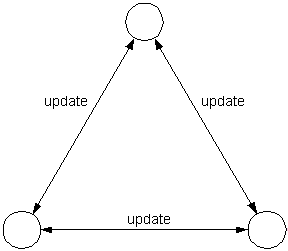
\includegraphics[scale = 0.7]{24/active.png}
	\caption{Схема активной репликации}
	\label{fig:active_repl}
\end{figure}

\textbf{Пассивная репликация (на англ. Primary-Backup Approach)} - каждый элемент (реплика) системы хранит копию состояния данных. Одна из реплик назначается главной. Операции чтения выполняются локально во всех узлах. Операции, модифицирующие состояние объекта, направляются главной реплике, которая, после выполнения метода, обновляет все остальные реплики. При выводе из строя главной реплики пользователь замечает проблемы с доступом к данным, до тех пор пока одна из запасных реплик не возьмет на себя роль главной. Данный метод обладает намного меньшим потреблением ресурсов и отсутствие большого количества избыточных коммуникаций и вычислений в сравнении с активной репликацией, и поэтому используется чаще.
\begin{figure}[H]
	\centering
	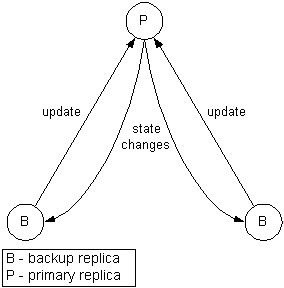
\includegraphics[scale = 0.7]{24/passive.png}
	\caption{Схема пассивной репликации}
	\label{fig:passive_repl}
\end{figure}



	

\newpage
\section {Билет 25. Модели логического разграничения доступа: мандатная, дискреционная, ролевая. Атрибутивная модель.}

\begin{center}
	\textit{\underline{Политика разграничения доступа}}
\end{center}

\textbf{Политика разграничения доступа} - набор правил, определяющий условия, при которых допускается выполнение той или иной операции над данными, т.е. отвечает на следующие вопросы: <<Кому? Что? И для каких данных можно сделать?>>\\

\textbf{Разграничение доступа} - техники реализации политики информационной безопасности. Существует два класса разграничения доступа:
\begin{itemize}
 \item \textbf{Физическое разграничение} - ограничение физического доступа к данным: закрытие помещений, изоляция устройств и т.д.
 \item \textbf{Логическое разграничение} - ограничение на уровне сущностей информационной системы (файлов, записей в БД, сетевого доступа).
\end{itemize}

Далее рассмотрим различные модели \textbf{логического разграничения}. Здесь тоже можно выделить два класса моделей:
\begin{enumerate}
	\item Проверка условий доступа ВО ВРЕМЯ выполнения конкретных операций над данными. 
	\item Проверка условий доступа ДО выполнения конкретных операций над данными.
\end{enumerate}

\textbf{Первый тип} проверок условий доступа может выполняться прямо в коде операции и например выглядеть следующим образом:
\begin{algorithm}
\begin{algorithmic}[H!]
	\If{(Условия доступа НЕ выполнены)}
	\State *Ошибка*
	\EndIf
	
	\State *Выполняем операцию*
\end{algorithmic}
\end{algorithm}


Данные проверки можно также реализовать за счет разных конструкций присущих разным языкам (Декораторы, Метаклассы - Python; Mixin'ы, Наследования - С++; и т.д). Также опишем достоинства и недостатки данного подхода.

\begin{figure}[H]
	\centering
	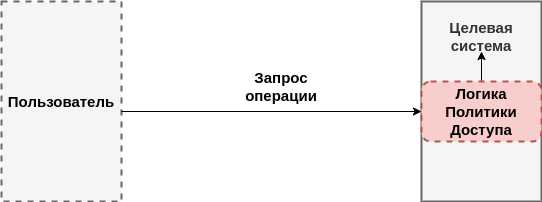
\includegraphics[scale = 0.7]{25/AC_in.png}
	\caption{Логика доступа внутри операции}
	\label{fig:ac_in}
\end{figure}


\begin{itemize}
	\item \textbf{Достоинства}:
	\begin{enumerate}
		\item Гибкость, так как можно производить любые вычисления и реализовывать сложную логику.
	\end{enumerate}
	\item \textbf{Недостатки}:
	\begin{enumerate}
		\item Логика политики распределена по исходному коду. Соответственно для ее изменения нужно менять значительную часть исходного кода операции.
		\item Невозможно анализировать <<корректность>> реализованной политики, так как она реализована на алгоритмически полном языке (или Тьюринг полном языке) то данная задача сводиться к нерешенной \href{https://clck.ru/pui5M}{<<проблеме остановки>>}. В связи с чем высока вероятность ошибки, которую очень сложно выявить.
	\end{enumerate}
\end{itemize}


\textbf{Второй тип} проверок условий доступа выделяет логику доступа в отдельную <<сущность>> и дает возможность реализовать ее на не алгоритмически полном языке.
\begin{itemize}
	\item \textbf{Достоинства}:
	\begin{enumerate}
		\item Вся логика содержится в одном месте и для ее изменения нужно менять малую часть кода.
		\item Из-за алгоритмической (Тьюринг) не полноты возможен анализ и верификация логики, в связи с чем количество сложно выявляемых ошибок стремиться к нулю.
	\end{enumerate}
	\item \textbf{Недостатки}:
	\begin{enumerate}
		\item Из-за алгоритмической (Тьюринг) не полноты возможно не получится реализовать все возможные варианты логики политики доступа.
	\end{enumerate}
\end{itemize}

\begin{figure}[H]
	\centering
	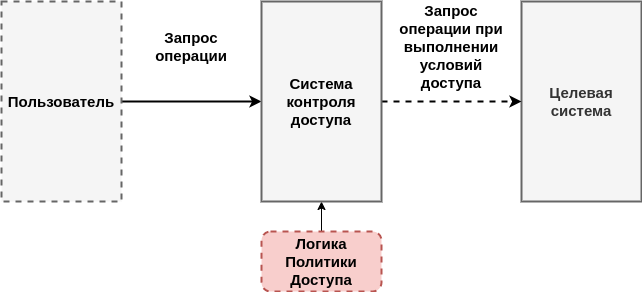
\includegraphics[scale = 0.7]{25/AC_out.png}
	\caption{Логика доступа вне операции}
	\label{fig:ac_out}
\end{figure}

На практике используются большое количество различных моделей политик разграничения доступа (DAC, MAC, RBAC, HBAC, IBAC, CBAC, ABAC, GBAC, ...). Рассмотрим несколько наиболее распространенных.

\begin{center}
	\textit{\underline{Мандатная (MAC)}}
\end{center}

\textbf{Мандатная, MAC(Mandatory Access Control)} - Принудительный контроль доступа. В модели \textbf{MAC} каждому объекту назначается метка конфиденциальности (Не секретно, для служебного пользования, секретно, совершенно секретно, и т.д.), а пользователю выдаются допуски. Данная модель используется в ядре ОС Linux и во многих других ОС к которым предъявляются высокие требования к безопастности, изменение меток как правило производится только администраторами. 

В данной модели на метках конфиденциальности и допусках пользователя вводится отношение порядка, например: $$\text{Не секретно} < \text {Для служебного пользования} < \text{Секретно} < \text {Совершенно секретно}$$

Причем должны выполняться следующие условия:
\begin{itemize}
	\item Пусть дана метка $m_i$, тогда для любых $m_j > m_i$ пользователь с допуском $m_i$ не имеет права ни на какие операции для данных с метками $m_j$.
	\item Пусть дана метка $m_i$, тогда для любых $m_j < m_i$ пользователь с допуском $m_i$ имеет право только на <<чтение>> данных с меткой $m_j$.
\end{itemize}

Из недостатков можно выделить невозможность предоставление доступа только к части данных в рамках одной метки, например нельзя дать доступ только к одной части документов с метками <<Совершенно секретно>> для пользователей с соответствующим доступом.

\begin{center}
	\textit{\underline{Дискреционная (DAC)}}
\end{center}

\textbf{Дискреционная, DAC(Discretionary Access Control)} - Избирательный контроль доступа. В модели \textbf{DAC} доступ к объекту осуществляется на основе матрицы доступа (например по столбцам все данные, а по строчкам все пользователи и в пересечении нужных строк и столбцов стоит метка обозначающая какой доступ разрешен/запрещен) или на основе списков управления доступом (список пользователей имеющих доступ к данным). Для каждой пары (субъект(пользователь) — объект(данные)) должно быть задано явное и недвусмысленное перечисление допустимых типов доступа (читать, писать и т. д.), то есть тех типов доступа, которые являются санкционированными для данного субъекта (индивида или группы индивидов) к данному ресурсу (объекту).

Возможны несколько подходов к построению дискреционного управления доступом:
\begin{itemize}
\item Каждый объект системы имеет привязанного к нему субъекта, называемого владельцем. Именно владелец устанавливает права доступа к объекту.
\item Система имеет одного выделенного субъекта — суперпользователя, который имеет право устанавливать права владения для всех остальных субъектов системы.
\item Субъект с определённым правом доступа может передать это право любому другому субъекту.
\end{itemize}

Возможны и смешанные варианты построения, когда одновременно в системе присутствуют как владельцы, устанавливающие права доступа к своим объектам, так и суперпользователь, имеющий возможность изменения прав для любого объекта и/или изменения его владельца. Именно такой смешанный вариант реализован в большинстве операционных систем, например Unix или Windows NT.

\begin{center}
	\textit{\underline{Ролевая (RBAC)}}
\end{center}

\textbf{Ролевая, RBAC (Role Based Access Control)} - Ролевой контроль доступа. Модель \textbf{RBAC} является развитием политики избирательного управления доступом (DAC), при этом права доступа субъектов системы на объекты группируются с учётом специфики их применения, образуя роли (Директор, Секретарь, Бухгалтер и т.д. ).

Формирование ролей призвано определить чёткие и понятные для пользователей компьютерной системы правила разграничения доступа. Ролевое разграничение доступа позволяет реализовать гибкие, изменяющиеся динамически в процессе функционирования компьютерной системы.

Такое разграничение доступа является составляющей многих современных компьютерных систем. Как правило, данный подход применяется в системах защиты СУБД, а отдельные элементы реализуются в сетевых операционных системах. Ролевой подход часто используется в системах, для пользователей которых чётко определён круг их должностных полномочий и обязанностей.

Так как привилегии не назначаются пользователям непосредственно и приобретаются ими только через свою роль (или роли), управление индивидуальными правами пользователя по сути сводится к назначению ему ролей. Это упрощает такие операции, как добавление пользователя или смена подразделения пользователем.

Для определения модели RBAC используются следующие соглашения:
\begin{itemize}
\item $S$ = Субъект = Человек или автоматизированный агент (множество пользователей);
\item $R$ = Роль  = Рабочая функция или название, которое определяется на уровне авторизации (множество ролей);
\item $P$ = Разрешения = Утверждения режима доступа к ресурсу (множество прав доступа на объекты системы);
\item $SE$ = Сессия = Соответствие между S, R и/или P
\item $SA$ = Назначение субъекта
\item $PA: R \to 2^p$ — функция, определяющая для каждой роли множество прав доступа; при этом для каждого $p \in P$ существует $r \in R$ такая, что $p \in PA(r)$;
\item $RH$ = Частично упорядоченная иерархия ролей. $RH$ может быть еще записана так: ≥
\item Один субъект может иметь несколько ролей.
\item Одну роль могут иметь несколько субъектов.
\item Одна роль может иметь несколько разрешений.
\item Одно разрешение может принадлежать нескольким ролям.
\end{itemize}


Роли назначаются субъектам, вследствие чего субъекты получают те или иные разрешения через роли. RBAC требует именно такого назначения, а не прямого назначения разрешений субъектам, иначе это приводит к сложно контролируемым отношениям между субъектами и разрешениям. На возможность наследования разрешений от противоположных ролей накладывается ограничительная норма, которая позволяет достичь надлежащего разделения режимов. Например, одному и тому же лицу может быть не позволено создать учётную запись для кого-то, а затем авторизоваться под этой учётной записью.

Используя нотацию теории множеств, $x ≥ y$ означает, что $x$ наследует разрешения $y$:
\begin{itemize}
\item $PA \subseteq P \times R$, при этом разрешения назначаются связям ролей в отношении «многие ко многим».
\item $SA \subseteq S \times R$, при этом субъекты назначаются связям ролей и субъектов в отношении «многие ко многим».
\item $RH \subseteq R \times R$
\end{itemize}

\begin{center}
	\textit{\underline{Атрибутивная (ABAC)}}
\end{center}

\textbf{Атрибутная, ABAC (Attribute Based Access Control)} - Атрибутный контроль доступа. Модель \textbf{ABAC} является развитием политики избирательного управления доступом (DAC) и политики ролевого контроля доступа. Рассматриваемый вид разграничения доступа даёт возможность создать огромное количество комбинаций условий для выражения различных политик. Например дать доступ Бухгалтеру на запись некоторых данных только в промежутке между 9 и 18 часов.



\newpage
\section {Билет 26. Конфиденциальные вычисления. Гомоморфное шифрование и многосторонние вычисления.}

\end{document}
